\documentclass[a4paper]{book}
\usepackage{makeidx}
\usepackage{graphicx}
\usepackage{multicol}
\usepackage{float}
\usepackage{listings}
\usepackage{color}
\usepackage{ifthen}
\usepackage[table]{xcolor}
\usepackage{textcomp}
\usepackage{alltt}
\usepackage{ifpdf}
\ifpdf
\usepackage[pdftex,
            pagebackref=true,
            colorlinks=true,
            linkcolor=blue,
            unicode
           ]{hyperref}
\else
\usepackage[ps2pdf,
            pagebackref=true,
            colorlinks=true,
            linkcolor=blue,
            unicode
           ]{hyperref}
\usepackage{pspicture}
\fi
\usepackage[utf8]{inputenc}
\usepackage{mathptmx}
\usepackage[scaled=.90]{helvet}
\usepackage{courier}
\usepackage{doxygen}
\lstset{language=C++,inputencoding=utf8,basicstyle=\footnotesize,breaklines=true,breakatwhitespace=true,tabsize=8,numbers=left }
\makeindex
\setcounter{tocdepth}{3}
\renewcommand{\footrulewidth}{0.4pt}
\begin{document}
\hypersetup{pageanchor=false}
\begin{titlepage}
\vspace*{7cm}
\begin{center}
{\Large Reference Manual}\\
\vspace*{1cm}
{\large Generated by Doxygen 1.7.3}\\
\vspace*{0.5cm}
{\small Tue Apr 30 2013 15:00:08}\\
\end{center}
\end{titlepage}
\clearemptydoublepage
\pagenumbering{roman}
\tableofcontents
\clearemptydoublepage
\pagenumbering{arabic}
\hypersetup{pageanchor=true}
\chapter{Class Index}
\section{Class Hierarchy}
This inheritance list is sorted roughly, but not completely, alphabetically:\begin{DoxyCompactList}
\item \contentsline{section}{app}{\pageref{structapp}}{}
\item \contentsline{section}{cl\_\-base}{\pageref{classcl__base}}{}
\begin{DoxyCompactList}
\item \contentsline{section}{cl\_\-app}{\pageref{classcl__app}}{}
\item \contentsline{section}{cl\_\-error}{\pageref{classcl__error}}{}
\item \contentsline{section}{cl\_\-error\_\-class}{\pageref{classcl__error__class}}{}
\item \contentsline{section}{cl\_\-event}{\pageref{classcl__event}}{}
\item \contentsline{section}{cl\_\-list}{\pageref{classcl__list}}{}
\begin{DoxyCompactList}
\item \contentsline{section}{cl\_\-sorted\_\-list}{\pageref{classcl__sorted__list}}{}
\begin{DoxyCompactList}
\item \contentsline{section}{cl\_\-options}{\pageref{classcl__options}}{}
\item \contentsline{section}{cl\_\-strings}{\pageref{classcl__strings}}{}
\begin{DoxyCompactList}
\item \contentsline{section}{cl\_\-ustrings}{\pageref{classcl__ustrings}}{}
\end{DoxyCompactList}
\end{DoxyCompactList}
\end{DoxyCompactList}
\item \contentsline{section}{cl\_\-option}{\pageref{classcl__option}}{}
\begin{DoxyCompactList}
\item \contentsline{section}{cl\_\-bool\_\-option}{\pageref{classcl__bool__option}}{}
\item \contentsline{section}{cl\_\-float\_\-option}{\pageref{classcl__float__option}}{}
\item \contentsline{section}{cl\_\-number\_\-option}{\pageref{classcl__number__option}}{}
\item \contentsline{section}{cl\_\-pointer\_\-option}{\pageref{classcl__pointer__option}}{}
\item \contentsline{section}{cl\_\-string\_\-option}{\pageref{classcl__string__option}}{}
\end{DoxyCompactList}
\item \contentsline{section}{cl\_\-optref}{\pageref{classcl__optref}}{}
\end{DoxyCompactList}
\item \contentsline{section}{cpu\_\-entry}{\pageref{structcpu__entry}}{}
\item \contentsline{section}{dis\_\-entry}{\pageref{structdis__entry}}{}
\item \contentsline{section}{id\_\-element}{\pageref{structid__element}}{}
\item \contentsline{section}{input\_\-args}{\pageref{structinput__args}}{}
\item \contentsline{section}{name\_\-entry}{\pageref{structname__entry}}{}
\item \contentsline{section}{option\_\-value}{\pageref{unionoption__value}}{}
\item \contentsline{section}{sim\_\-args}{\pageref{structsim__args}}{}
\end{DoxyCompactList}

\chapter{Class Index}
\section{Class List}
Here are the classes, structs, unions and interfaces with brief descriptions:\begin{DoxyCompactList}
\item\contentsline{section}{\hyperlink{structapp}{app} }{\pageref{structapp}}{}
\item\contentsline{section}{\hyperlink{classcl__app}{cl\_\-app} }{\pageref{classcl__app}}{}
\item\contentsline{section}{\hyperlink{classcl__base}{cl\_\-base} }{\pageref{classcl__base}}{}
\item\contentsline{section}{\hyperlink{classcl__bool__option}{cl\_\-bool\_\-option} }{\pageref{classcl__bool__option}}{}
\item\contentsline{section}{\hyperlink{classcl__error}{cl\_\-error} }{\pageref{classcl__error}}{}
\item\contentsline{section}{\hyperlink{classcl__error__class}{cl\_\-error\_\-class} }{\pageref{classcl__error__class}}{}
\item\contentsline{section}{\hyperlink{classcl__event}{cl\_\-event} }{\pageref{classcl__event}}{}
\item\contentsline{section}{\hyperlink{classcl__float__option}{cl\_\-float\_\-option} }{\pageref{classcl__float__option}}{}
\item\contentsline{section}{\hyperlink{classcl__list}{cl\_\-list} }{\pageref{classcl__list}}{}
\item\contentsline{section}{\hyperlink{classcl__number__option}{cl\_\-number\_\-option} }{\pageref{classcl__number__option}}{}
\item\contentsline{section}{\hyperlink{classcl__option}{cl\_\-option} }{\pageref{classcl__option}}{}
\item\contentsline{section}{\hyperlink{classcl__options}{cl\_\-options} }{\pageref{classcl__options}}{}
\item\contentsline{section}{\hyperlink{classcl__optref}{cl\_\-optref} }{\pageref{classcl__optref}}{}
\item\contentsline{section}{\hyperlink{classcl__pointer__option}{cl\_\-pointer\_\-option} }{\pageref{classcl__pointer__option}}{}
\item\contentsline{section}{\hyperlink{classcl__sorted__list}{cl\_\-sorted\_\-list} }{\pageref{classcl__sorted__list}}{}
\item\contentsline{section}{\hyperlink{classcl__string__option}{cl\_\-string\_\-option} }{\pageref{classcl__string__option}}{}
\item\contentsline{section}{\hyperlink{classcl__strings}{cl\_\-strings} }{\pageref{classcl__strings}}{}
\item\contentsline{section}{\hyperlink{classcl__ustrings}{cl\_\-ustrings} }{\pageref{classcl__ustrings}}{}
\item\contentsline{section}{\hyperlink{structcpu__entry}{cpu\_\-entry} }{\pageref{structcpu__entry}}{}
\item\contentsline{section}{\hyperlink{structdis__entry}{dis\_\-entry} }{\pageref{structdis__entry}}{}
\item\contentsline{section}{\hyperlink{structid__element}{id\_\-element} }{\pageref{structid__element}}{}
\item\contentsline{section}{\hyperlink{structinput__args}{input\_\-args} }{\pageref{structinput__args}}{}
\item\contentsline{section}{\hyperlink{structname__entry}{name\_\-entry} }{\pageref{structname__entry}}{}
\item\contentsline{section}{\hyperlink{unionoption__value}{option\_\-value} }{\pageref{unionoption__value}}{}
\item\contentsline{section}{\hyperlink{structsim__args}{sim\_\-args} }{\pageref{structsim__args}}{}
\end{DoxyCompactList}

\chapter{Class Documentation}
\hypertarget{structapp}{
\section{app Struct Reference}
\label{structapp}\index{app@{app}}
}
\subsection*{Public Attributes}
\begin{DoxyCompactItemize}
\item 
\hypertarget{structapp_a78260cd49a2b5fb996eaccd48a0e99c7}{
long {\bfseries PC}}
\label{structapp_a78260cd49a2b5fb996eaccd48a0e99c7}

\item 
\hypertarget{structapp_ad56e86d53459ffc454a21f385d7a1f65}{
bool {\bfseries simulating}}
\label{structapp_ad56e86d53459ffc454a21f385d7a1f65}

\end{DoxyCompactItemize}


The documentation for this struct was generated from the following file:\begin{DoxyCompactItemize}
\item 
ptt.cc\end{DoxyCompactItemize}

\hypertarget{classcl__app}{
\section{cl\_\-app Class Reference}
\label{classcl__app}\index{cl\_\-app@{cl\_\-app}}
}
Inheritance diagram for cl\_\-app:\begin{figure}[H]
\begin{center}
\leavevmode
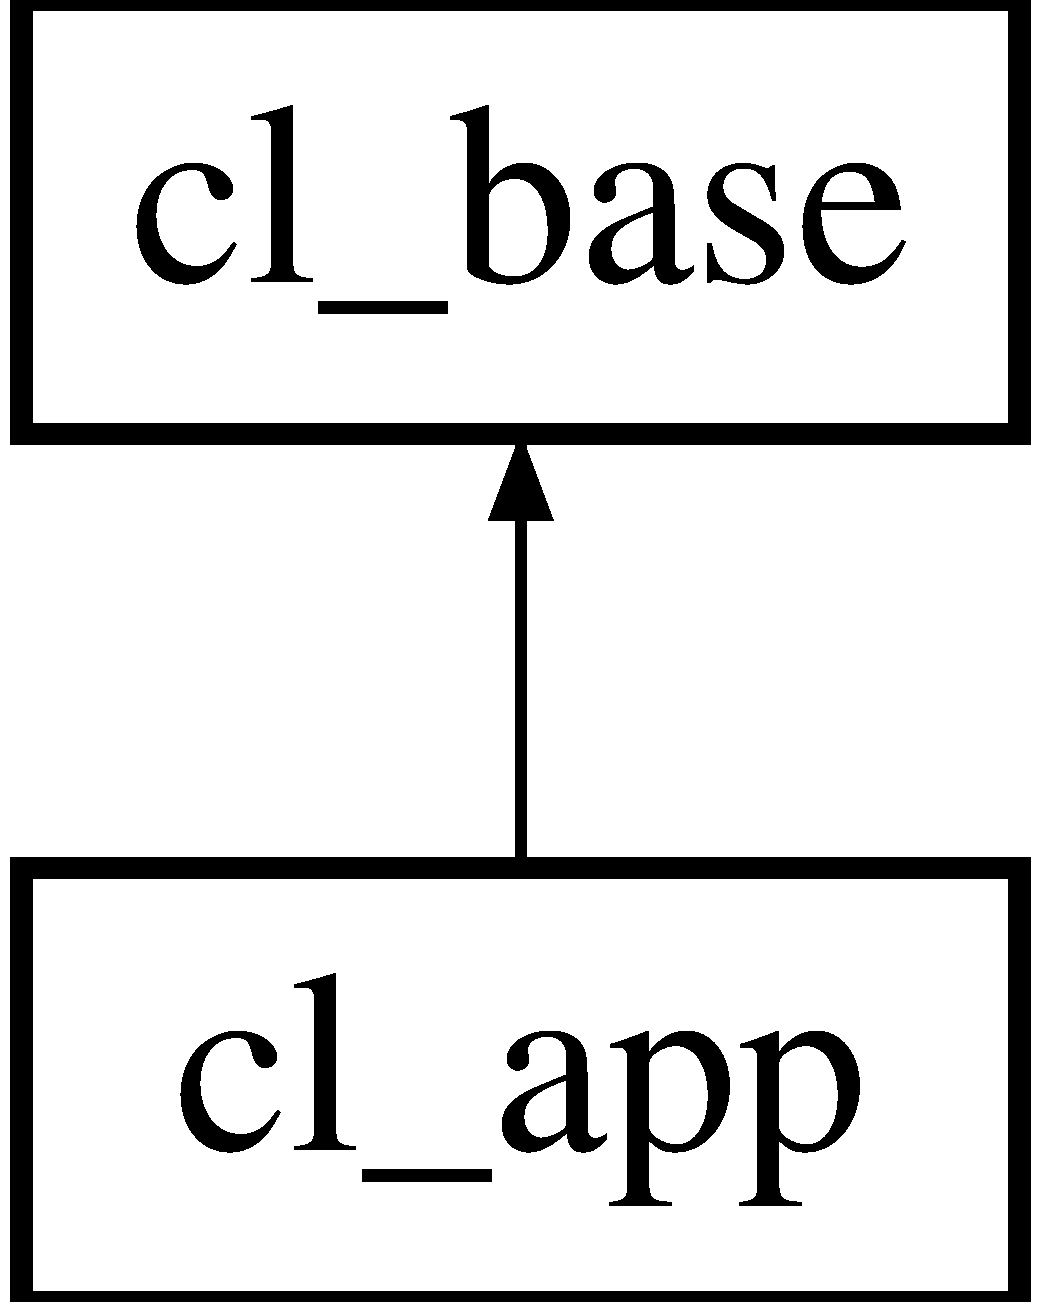
\includegraphics[height=2.000000cm]{classcl__app}
\end{center}
\end{figure}
\subsection*{Public Member Functions}
\begin{DoxyCompactItemize}
\item 
\hypertarget{classcl__app_af1ae3d613ed5a8cfeee50768f23f0d18}{
virtual int {\bfseries init} (int argc, char $\ast$argv\mbox{[}$\,$\mbox{]})}
\label{classcl__app_af1ae3d613ed5a8cfeee50768f23f0d18}

\item 
\hypertarget{classcl__app_aafdec4ecc1592f745766da411de937dd}{
virtual int {\bfseries run} (void)}
\label{classcl__app_aafdec4ecc1592f745766da411de937dd}

\item 
\hypertarget{classcl__app_a1f2caf1fbc15c4f2d8100f973f6ab909}{
virtual void {\bfseries done} (void)}
\label{classcl__app_a1f2caf1fbc15c4f2d8100f973f6ab909}

\item 
\hypertarget{classcl__app_adbf148a46af4915fa533c8483f67f9df}{
class cl\_\-sim $\ast$ {\bfseries get\_\-sim} (void)}
\label{classcl__app_adbf148a46af4915fa533c8483f67f9df}

\item 
\hypertarget{classcl__app_a22097a1116d7ebaff1142ad200f95a0e}{
class cl\_\-uc $\ast$ {\bfseries get\_\-uc} (void)}
\label{classcl__app_a22097a1116d7ebaff1142ad200f95a0e}

\item 
\hypertarget{classcl__app_ac22477ce4a85ab0ef94188d130f890a5}{
class cl\_\-commander $\ast$ {\bfseries get\_\-commander} (void)}
\label{classcl__app_ac22477ce4a85ab0ef94188d130f890a5}

\item 
\hypertarget{classcl__app_a4a3f00592cc63fa5736e3bba1557c566}{
virtual class cl\_\-cmd $\ast$ {\bfseries get\_\-cmd} (class cl\_\-cmdline $\ast$cmdline)}
\label{classcl__app_a4a3f00592cc63fa5736e3bba1557c566}

\item 
\hypertarget{classcl__app_a6add6e2648d57e7d7383b9320179c74b}{
virtual void {\bfseries set\_\-simulator} (class cl\_\-sim $\ast$simulator)}
\label{classcl__app_a6add6e2648d57e7d7383b9320179c74b}

\item 
\hypertarget{classcl__app_acd888273e848fe87151e0781da93895f}{
virtual void {\bfseries remove\_\-simulator} (void)}
\label{classcl__app_acd888273e848fe87151e0781da93895f}

\item 
\hypertarget{classcl__app_a0a68e3a0beb3daa59a166bd1578383fe}{
virtual int {\bfseries dd\_\-printf} (char $\ast$format,...)}
\label{classcl__app_a0a68e3a0beb3daa59a166bd1578383fe}

\item 
\hypertarget{classcl__app_a52bed4fba7c628a661e0455a2e091863}{
virtual int {\bfseries debug} (char $\ast$format,...)}
\label{classcl__app_a52bed4fba7c628a661e0455a2e091863}

\end{DoxyCompactItemize}
\subsection*{Public Attributes}
\begin{DoxyCompactItemize}
\item 
\hypertarget{classcl__app_a94eb36e019d36f6336ad62862c1a25c2}{
class cl\_\-sim $\ast$ {\bfseries sim}}
\label{classcl__app_a94eb36e019d36f6336ad62862c1a25c2}

\item 
\hypertarget{classcl__app_a4882666f7131e7b1e81cc9fc8fca6403}{
class \hyperlink{classcl__ustrings}{cl\_\-ustrings} $\ast$ {\bfseries in\_\-files}}
\label{classcl__app_a4882666f7131e7b1e81cc9fc8fca6403}

\item 
\hypertarget{classcl__app_aba6e14ee58a1edb482a1b405c0cfd149}{
class \hyperlink{classcl__options}{cl\_\-options} $\ast$ {\bfseries options}}
\label{classcl__app_aba6e14ee58a1edb482a1b405c0cfd149}

\item 
\hypertarget{classcl__app_af9769001edcf99f03f1d93b2e7b4e589}{
int {\bfseries going}}
\label{classcl__app_af9769001edcf99f03f1d93b2e7b4e589}

\end{DoxyCompactItemize}
\subsection*{Protected Member Functions}
\begin{DoxyCompactItemize}
\item 
\hypertarget{classcl__app_a8b96791b0d866b1f3ffa2b789c65f193}{
virtual int {\bfseries proc\_\-arguments} (int argc, char $\ast$argv\mbox{[}$\,$\mbox{]})}
\label{classcl__app_a8b96791b0d866b1f3ffa2b789c65f193}

\item 
\hypertarget{classcl__app_a8d483117b05cc19fc826fa47ec024e9f}{
virtual void {\bfseries build\_\-cmdset} (class cl\_\-cmdset $\ast$cs)}
\label{classcl__app_a8d483117b05cc19fc826fa47ec024e9f}

\item 
\hypertarget{classcl__app_af661a94adb2681eb930f2d4bcd0724e6}{
virtual void {\bfseries mk\_\-options} (void)}
\label{classcl__app_af661a94adb2681eb930f2d4bcd0724e6}

\end{DoxyCompactItemize}
\subsection*{Protected Attributes}
\begin{DoxyCompactItemize}
\item 
\hypertarget{classcl__app_acb07f7525b77148df0d6e73587d6dbea}{
class cl\_\-commander $\ast$ {\bfseries commander}}
\label{classcl__app_acb07f7525b77148df0d6e73587d6dbea}

\end{DoxyCompactItemize}


The documentation for this class was generated from the following files:\begin{DoxyCompactItemize}
\item 
appcl.h\item 
app.cc\end{DoxyCompactItemize}

\hypertarget{classcl__base}{
\section{cl\_\-base Class Reference}
\label{classcl__base}\index{cl\_\-base@{cl\_\-base}}
}
Inheritance diagram for cl\_\-base:\begin{figure}[H]
\begin{center}
\leavevmode
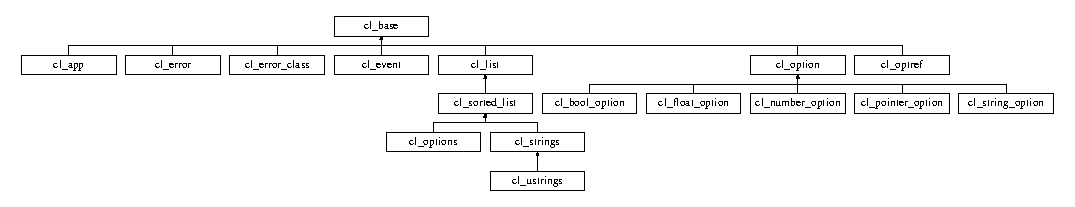
\includegraphics[height=2.333333cm]{classcl__base}
\end{center}
\end{figure}
\subsection*{Public Member Functions}
\begin{DoxyCompactItemize}
\item 
\hypertarget{classcl__base_a3804b6d8f2ce3a5e5b040a0346c5df12}{
virtual int {\bfseries init} (void)}
\label{classcl__base_a3804b6d8f2ce3a5e5b040a0346c5df12}

\item 
\hypertarget{classcl__base_a42251e19372c87758751e7793435b5b9}{
virtual char $\ast$ {\bfseries get\_\-name} (void)}
\label{classcl__base_a42251e19372c87758751e7793435b5b9}

\item 
\hypertarget{classcl__base_ac28e9c4747af317608f3a3d9ced2c73e}{
virtual char $\ast$ {\bfseries get\_\-name} (char $\ast$def)}
\label{classcl__base_ac28e9c4747af317608f3a3d9ced2c73e}

\item 
\hypertarget{classcl__base_aec39c1134181cfb60560c6ac83cedd6f}{
virtual bool {\bfseries have\_\-name} (void)}
\label{classcl__base_aec39c1134181cfb60560c6ac83cedd6f}

\item 
\hypertarget{classcl__base_af2a6ef67766f771763287e8db8abc559}{
virtual bool {\bfseries have\_\-real\_\-name} (void)}
\label{classcl__base_af2a6ef67766f771763287e8db8abc559}

\item 
\hypertarget{classcl__base_aab1d4c35918cc5fbd716580866a86094}{
char $\ast$ {\bfseries set\_\-name} (char $\ast$new\_\-name)}
\label{classcl__base_aab1d4c35918cc5fbd716580866a86094}

\item 
\hypertarget{classcl__base_a80c98cfa1463a93e2b587840e00a1d22}{
char $\ast$ {\bfseries set\_\-name} (char $\ast$new\_\-name, char $\ast$def\_\-name)}
\label{classcl__base_a80c98cfa1463a93e2b587840e00a1d22}

\item 
\hypertarget{classcl__base_a0369f79f3218534fd46ebeb82e0c7b87}{
bool {\bfseries is\_\-named} (char $\ast$the\_\-name)}
\label{classcl__base_a0369f79f3218534fd46ebeb82e0c7b87}

\item 
\hypertarget{classcl__base_af5cdd39f8c4e0e456a9f02f6f9244bac}{
bool {\bfseries is\_\-inamed} (char $\ast$the\_\-name)}
\label{classcl__base_af5cdd39f8c4e0e456a9f02f6f9244bac}

\item 
\hypertarget{classcl__base_a9798c52f642c89b813e3535687948f79}{
class \hyperlink{classcl__base}{cl\_\-base} $\ast$ {\bfseries get\_\-parent} (void)}
\label{classcl__base_a9798c52f642c89b813e3535687948f79}

\item 
\hypertarget{classcl__base_a018e2c1c6ef01ca6576f72fbef615106}{
int {\bfseries nuof\_\-children} (void)}
\label{classcl__base_a018e2c1c6ef01ca6576f72fbef615106}

\item 
\hypertarget{classcl__base_a87e97f59dfbba7fcd46255ddd856116c}{
virtual void {\bfseries add\_\-child} (class \hyperlink{classcl__base}{cl\_\-base} $\ast$child)}
\label{classcl__base_a87e97f59dfbba7fcd46255ddd856116c}

\item 
\hypertarget{classcl__base_ab07d05ca13369e1e38a0654abf3d048a}{
virtual void {\bfseries remove\_\-child} (class \hyperlink{classcl__base}{cl\_\-base} $\ast$child)}
\label{classcl__base_ab07d05ca13369e1e38a0654abf3d048a}

\item 
\hypertarget{classcl__base_a8cbaea6347e76bf511c7ed35b2b11e71}{
virtual void {\bfseries remove\_\-from\_\-chain} (void)}
\label{classcl__base_a8cbaea6347e76bf511c7ed35b2b11e71}

\item 
\hypertarget{classcl__base_accdf15ec0a9152dab6cc1138e11a8f14}{
virtual void {\bfseries unlink} (void)}
\label{classcl__base_accdf15ec0a9152dab6cc1138e11a8f14}

\item 
\hypertarget{classcl__base_ae70ac645f46b028ebfd952e73a3dec65}{
virtual class \hyperlink{classcl__base}{cl\_\-base} $\ast$ {\bfseries first\_\-child} (void)}
\label{classcl__base_ae70ac645f46b028ebfd952e73a3dec65}

\item 
\hypertarget{classcl__base_af231ce008f9244729f990bdd123e36cf}{
virtual class \hyperlink{classcl__base}{cl\_\-base} $\ast$ {\bfseries next\_\-child} (class \hyperlink{classcl__base}{cl\_\-base} $\ast$child)}
\label{classcl__base_af231ce008f9244729f990bdd123e36cf}

\item 
\hypertarget{classcl__base_a4bdbcda582c2949ae0afd9383b65bb73}{
virtual bool {\bfseries handle\_\-event} (class \hyperlink{classcl__event}{cl\_\-event} \&event)}
\label{classcl__base_a4bdbcda582c2949ae0afd9383b65bb73}

\item 
\hypertarget{classcl__base_ae56fabf74193c0e4bbd96d96eecda2bb}{
virtual bool {\bfseries pass\_\-event\_\-down} (class \hyperlink{classcl__event}{cl\_\-event} \&event)}
\label{classcl__base_ae56fabf74193c0e4bbd96d96eecda2bb}

\end{DoxyCompactItemize}


The documentation for this class was generated from the following files:\begin{DoxyCompactItemize}
\item 
pobjcl.h\item 
pobj.cc\end{DoxyCompactItemize}

\hypertarget{classcl__bool__option}{
\section{cl\_\-bool\_\-option Class Reference}
\label{classcl__bool__option}\index{cl\_\-bool\_\-option@{cl\_\-bool\_\-option}}
}
Inheritance diagram for cl\_\-bool\_\-option:\begin{figure}[H]
\begin{center}
\leavevmode
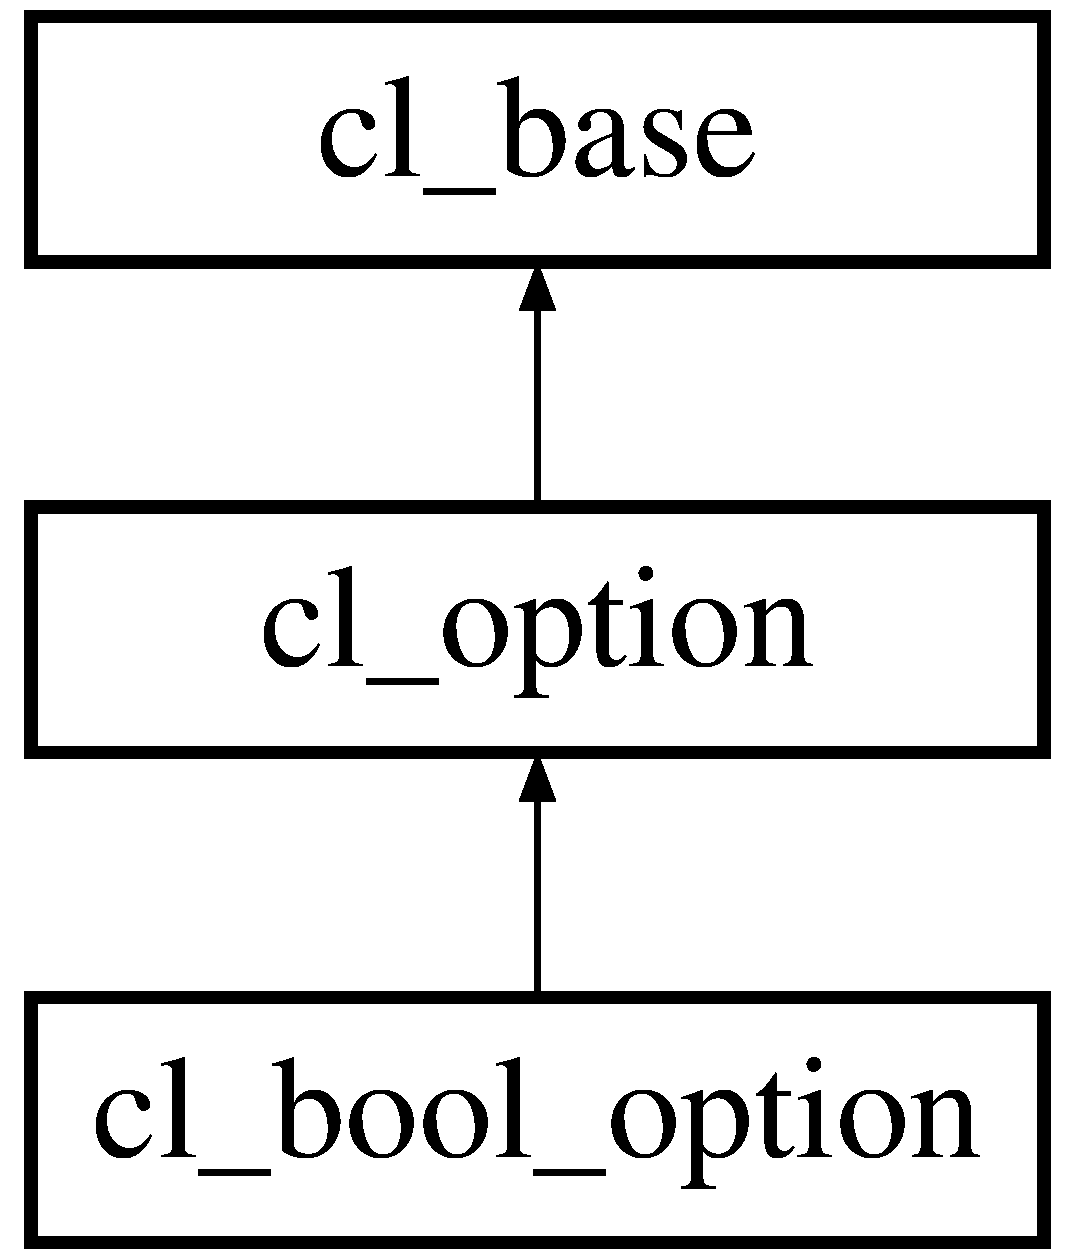
\includegraphics[height=3.000000cm]{classcl__bool__option}
\end{center}
\end{figure}
\subsection*{Public Member Functions}
\begin{DoxyCompactItemize}
\item 
\hypertarget{classcl__bool__option_a6de8128dfa335f981c87d34b41ad1560}{
{\bfseries cl\_\-bool\_\-option} (class \hyperlink{classcl__base}{cl\_\-base} $\ast$the\_\-creator, char $\ast$aname, char $\ast$Ihelp)}
\label{classcl__bool__option_a6de8128dfa335f981c87d34b41ad1560}

\item 
virtual void \hyperlink{classcl__bool__option_ab7183b00fb532bef27c70e20cafe3c3a}{print} (class cl\_\-console $\ast$con)
\item 
\hypertarget{classcl__bool__option_a9d211d1a851c8e3e5f4973c93050fe7b}{
virtual char $\ast$ {\bfseries get\_\-type\_\-name} (void)}
\label{classcl__bool__option_a9d211d1a851c8e3e5f4973c93050fe7b}

\item 
virtual void \hyperlink{classcl__bool__option_a79613291ae04d9b7119e6014a2ba4c72}{set\_\-value} (char $\ast$s)
\end{DoxyCompactItemize}


\subsection{Member Function Documentation}
\hypertarget{classcl__bool__option_ab7183b00fb532bef27c70e20cafe3c3a}{
\index{cl\_\-bool\_\-option@{cl\_\-bool\_\-option}!print@{print}}
\index{print@{print}!cl_bool_option@{cl\_\-bool\_\-option}}
\subsubsection[{print}]{\setlength{\rightskip}{0pt plus 5cm}void cl\_\-bool\_\-option::print (
\begin{DoxyParamCaption}
\item[{class cl\_\-console $\ast$}]{con}
\end{DoxyParamCaption}
)\hspace{0.3cm}{\ttfamily  \mbox{[}virtual\mbox{]}}}}
\label{classcl__bool__option_ab7183b00fb532bef27c70e20cafe3c3a}


(bool $\ast$)option 



Reimplemented from \hyperlink{classcl__option}{cl\_\-option}.

\hypertarget{classcl__bool__option_a79613291ae04d9b7119e6014a2ba4c72}{
\index{cl\_\-bool\_\-option@{cl\_\-bool\_\-option}!set\_\-value@{set\_\-value}}
\index{set\_\-value@{set\_\-value}!cl_bool_option@{cl\_\-bool\_\-option}}
\subsubsection[{set\_\-value}]{\setlength{\rightskip}{0pt plus 5cm}void cl\_\-bool\_\-option::set\_\-value (
\begin{DoxyParamCaption}
\item[{char $\ast$}]{s}
\end{DoxyParamCaption}
)\hspace{0.3cm}{\ttfamily  \mbox{[}virtual\mbox{]}}}}
\label{classcl__bool__option_a79613291ae04d9b7119e6014a2ba4c72}


(bool $\ast$)option=

(bool $\ast$)option= 



Reimplemented from \hyperlink{classcl__option}{cl\_\-option}.



The documentation for this class was generated from the following files:\begin{DoxyCompactItemize}
\item 
optioncl.h\item 
option.cc\end{DoxyCompactItemize}

\hypertarget{classcl__error}{
\section{cl\_\-error Class Reference}
\label{classcl__error}\index{cl\_\-error@{cl\_\-error}}
}
Inheritance diagram for cl\_\-error:\begin{figure}[H]
\begin{center}
\leavevmode
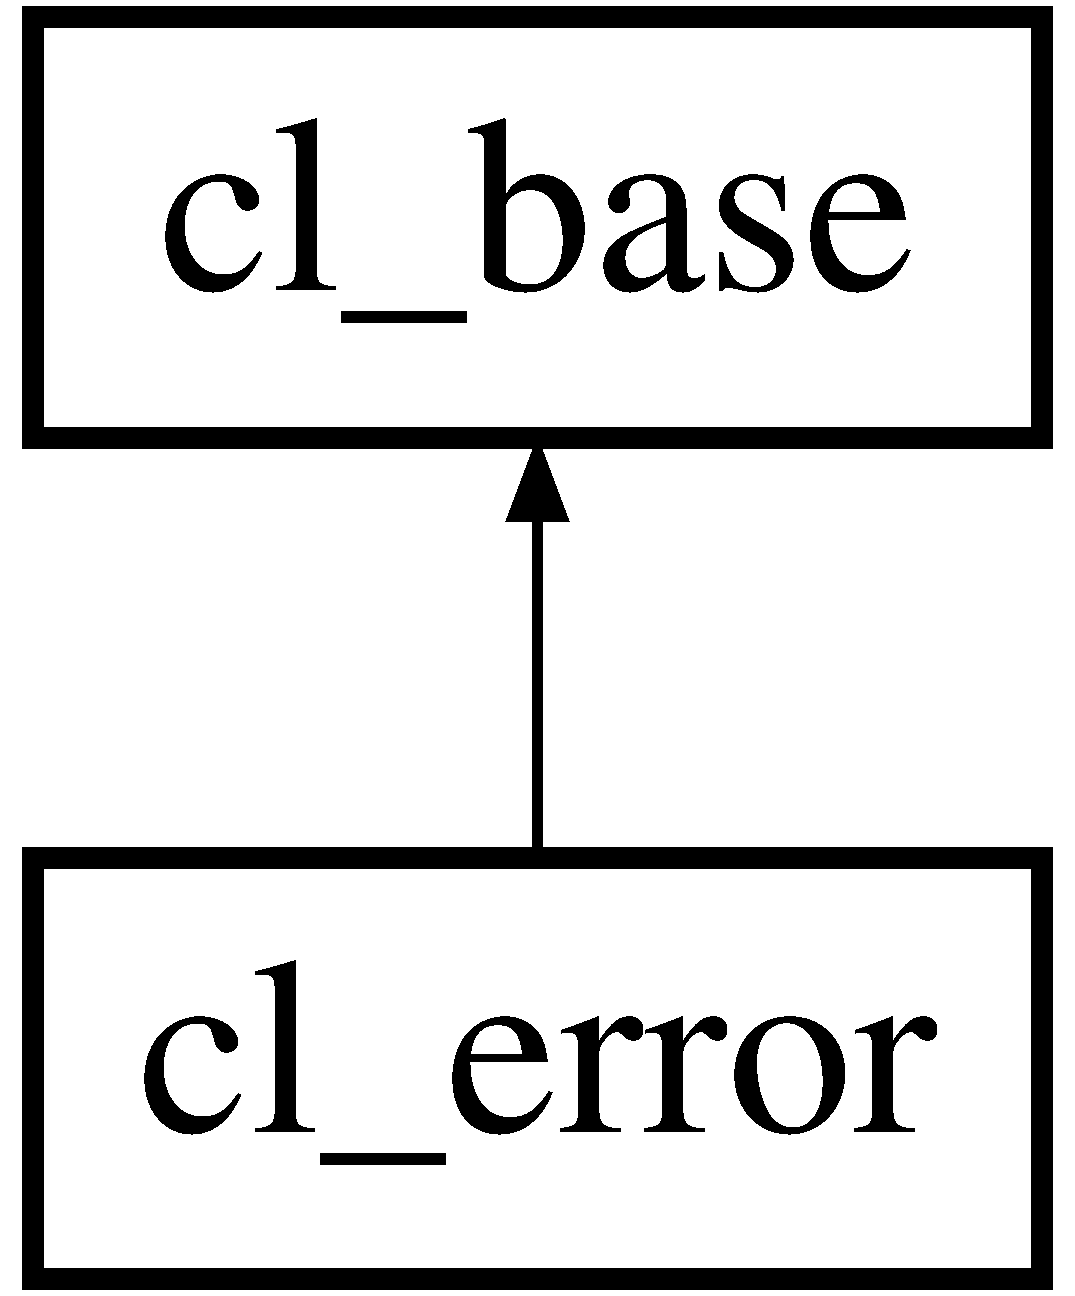
\includegraphics[height=2.000000cm]{classcl__error}
\end{center}
\end{figure}
\subsection*{Public Member Functions}
\begin{DoxyCompactItemize}
\item 
\hypertarget{classcl__error_aa55b52c6ccb658cfe1daebcda9efb5c9}{
virtual int {\bfseries init} (void)}
\label{classcl__error_aa55b52c6ccb658cfe1daebcda9efb5c9}

\item 
\hypertarget{classcl__error_a9ffc63267988da888ddf5bd4a4a57c76}{
virtual enum error\_\-type {\bfseries get\_\-type} (void)}
\label{classcl__error_a9ffc63267988da888ddf5bd4a4a57c76}

\item 
\hypertarget{classcl__error_a7e01970b4abc4b60c5f14cd60ece26fe}{
virtual enum error\_\-on\_\-off {\bfseries get\_\-on} (void)}
\label{classcl__error_a7e01970b4abc4b60c5f14cd60ece26fe}

\item 
\hypertarget{classcl__error_a69d8f21cc6f46aa5af32d795dc17d532}{
virtual bool {\bfseries is\_\-on} (void)}
\label{classcl__error_a69d8f21cc6f46aa5af32d795dc17d532}

\item 
\hypertarget{classcl__error_a41042138fb165126fb471da556261547}{
virtual class \hyperlink{classcl__error__class}{cl\_\-error\_\-class} $\ast$ {\bfseries get\_\-class} (void)}
\label{classcl__error_a41042138fb165126fb471da556261547}

\item 
\hypertarget{classcl__error_a56bdc8cfbfd3520f32e5696e5261d54e}{
virtual void {\bfseries print} (class cl\_\-commander $\ast$c)}
\label{classcl__error_a56bdc8cfbfd3520f32e5696e5261d54e}

\item 
\hypertarget{classcl__error_a9cdcd9d514e68985d84fa3e98cbfdc93}{
virtual char $\ast$ {\bfseries get\_\-type\_\-name} ()}
\label{classcl__error_a9cdcd9d514e68985d84fa3e98cbfdc93}

\end{DoxyCompactItemize}
\subsection*{Public Attributes}
\begin{DoxyCompactItemize}
\item 
\hypertarget{classcl__error_ab16e70c466947b908505113084543da8}{
bool {\bfseries inst}}
\label{classcl__error_ab16e70c466947b908505113084543da8}

\item 
\hypertarget{classcl__error_ab5b1cfac39b6c935634ed1a990887cb9}{
t\_\-addr {\bfseries PC}}
\label{classcl__error_ab5b1cfac39b6c935634ed1a990887cb9}

\end{DoxyCompactItemize}
\subsection*{Protected Attributes}
\begin{DoxyCompactItemize}
\item 
\hypertarget{classcl__error_ad44de3601a2155ceb126abb477de9c61}{
class \hyperlink{classcl__error__class}{cl\_\-error\_\-class} $\ast$ {\bfseries classification}}
\label{classcl__error_ad44de3601a2155ceb126abb477de9c61}

\end{DoxyCompactItemize}


The documentation for this class was generated from the following files:\begin{DoxyCompactItemize}
\item 
errorcl.h\item 
error.cc\end{DoxyCompactItemize}

\hypertarget{classcl__error__class}{
\section{cl\_\-error\_\-class Class Reference}
\label{classcl__error__class}\index{cl\_\-error\_\-class@{cl\_\-error\_\-class}}
}
Inheritance diagram for cl\_\-error\_\-class:\begin{figure}[H]
\begin{center}
\leavevmode
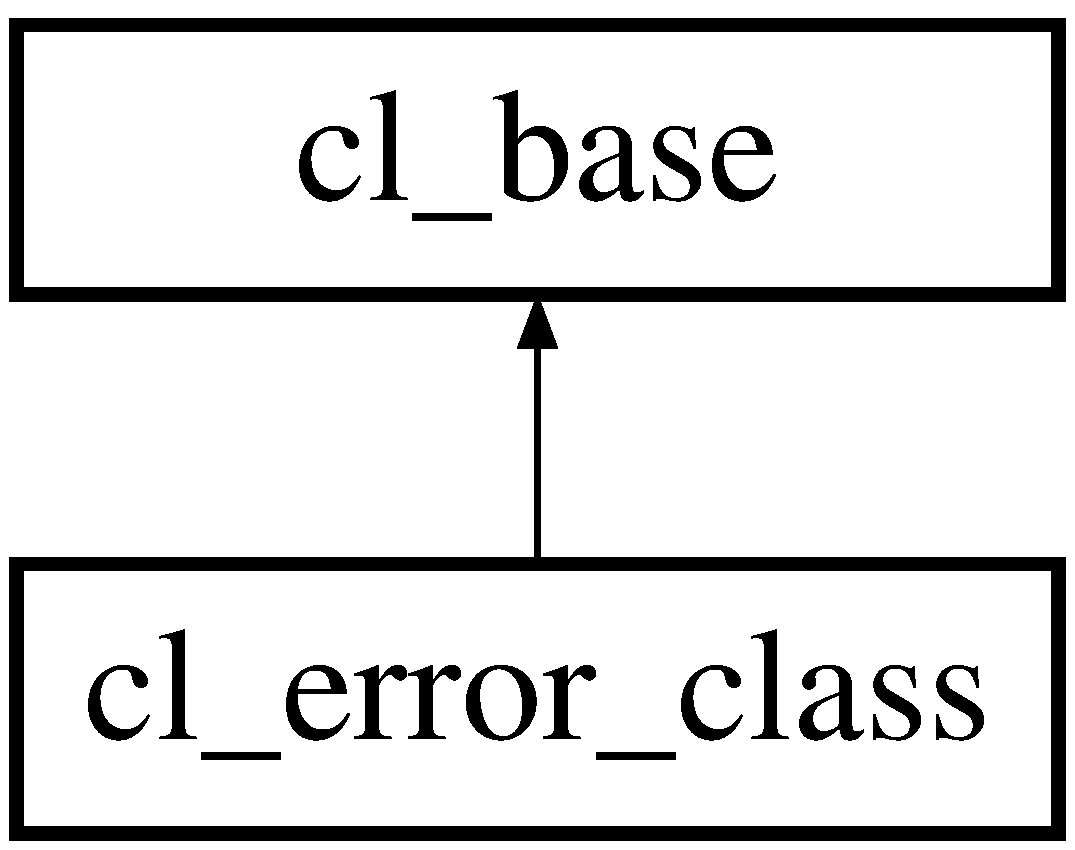
\includegraphics[height=2.000000cm]{classcl__error__class}
\end{center}
\end{figure}
\subsection*{Public Member Functions}
\begin{DoxyCompactItemize}
\item 
\hypertarget{classcl__error__class_a5d5f65aa751faed9295ae65dfa4e7a9e}{
{\bfseries cl\_\-error\_\-class} (enum error\_\-type typ, char $\ast$aname)}
\label{classcl__error__class_a5d5f65aa751faed9295ae65dfa4e7a9e}

\item 
\hypertarget{classcl__error__class_ae9236194853fde69cfe414bb1c6bc949}{
{\bfseries cl\_\-error\_\-class} (enum error\_\-type typ, char $\ast$aname, enum error\_\-on\_\-off be\_\-on)}
\label{classcl__error__class_ae9236194853fde69cfe414bb1c6bc949}

\item 
\hypertarget{classcl__error__class_adc00bc6c1fd8449a8d17f50acd35d9f5}{
{\bfseries cl\_\-error\_\-class} (enum error\_\-type typ, char $\ast$aname, class \hyperlink{classcl__error__class}{cl\_\-error\_\-class} $\ast$parent)}
\label{classcl__error__class_adc00bc6c1fd8449a8d17f50acd35d9f5}

\item 
\hypertarget{classcl__error__class_acaaf22d054293fb0b74909aa8be31290}{
{\bfseries cl\_\-error\_\-class} (enum error\_\-type typ, char $\ast$aname, class \hyperlink{classcl__error__class}{cl\_\-error\_\-class} $\ast$parent, enum error\_\-on\_\-off be\_\-on)}
\label{classcl__error__class_acaaf22d054293fb0b74909aa8be31290}

\item 
\hypertarget{classcl__error__class_a049290442ef81be14ba866f0c07d92ab}{
enum error\_\-on\_\-off {\bfseries get\_\-on} (void)}
\label{classcl__error__class_a049290442ef81be14ba866f0c07d92ab}

\item 
\hypertarget{classcl__error__class_a557020a680f757eecf9ca96eb118e8f4}{
void {\bfseries set\_\-on} (enum error\_\-on\_\-off val)}
\label{classcl__error__class_a557020a680f757eecf9ca96eb118e8f4}

\item 
\hypertarget{classcl__error__class_a3b08926a0574a8957b3b70e1ffe61ae3}{
bool {\bfseries is\_\-on} (void)}
\label{classcl__error__class_a3b08926a0574a8957b3b70e1ffe61ae3}

\item 
\hypertarget{classcl__error__class_acb9b042b5e8c868bc8e8d3774bde85cb}{
enum error\_\-type {\bfseries get\_\-type} (void)}
\label{classcl__error__class_acb9b042b5e8c868bc8e8d3774bde85cb}

\item 
\hypertarget{classcl__error__class_a02382dfc36598bc350297ce420451105}{
char $\ast$ {\bfseries get\_\-type\_\-name} (void)}
\label{classcl__error__class_a02382dfc36598bc350297ce420451105}

\end{DoxyCompactItemize}
\subsection*{Protected Attributes}
\begin{DoxyCompactItemize}
\item 
\hypertarget{classcl__error__class_ad3b9534254fe8c25604bc204b6f71c8c}{
enum error\_\-type {\bfseries type}}
\label{classcl__error__class_ad3b9534254fe8c25604bc204b6f71c8c}

\item 
\hypertarget{classcl__error__class_a546d6f340248ee3b04b81b6b66e689ea}{
enum error\_\-on\_\-off {\bfseries on}}
\label{classcl__error__class_a546d6f340248ee3b04b81b6b66e689ea}

\end{DoxyCompactItemize}


The documentation for this class was generated from the following files:\begin{DoxyCompactItemize}
\item 
errorcl.h\item 
error.cc\end{DoxyCompactItemize}

\hypertarget{classcl__event}{
\section{cl\_\-event Class Reference}
\label{classcl__event}\index{cl\_\-event@{cl\_\-event}}
}
Inheritance diagram for cl\_\-event:\begin{figure}[H]
\begin{center}
\leavevmode
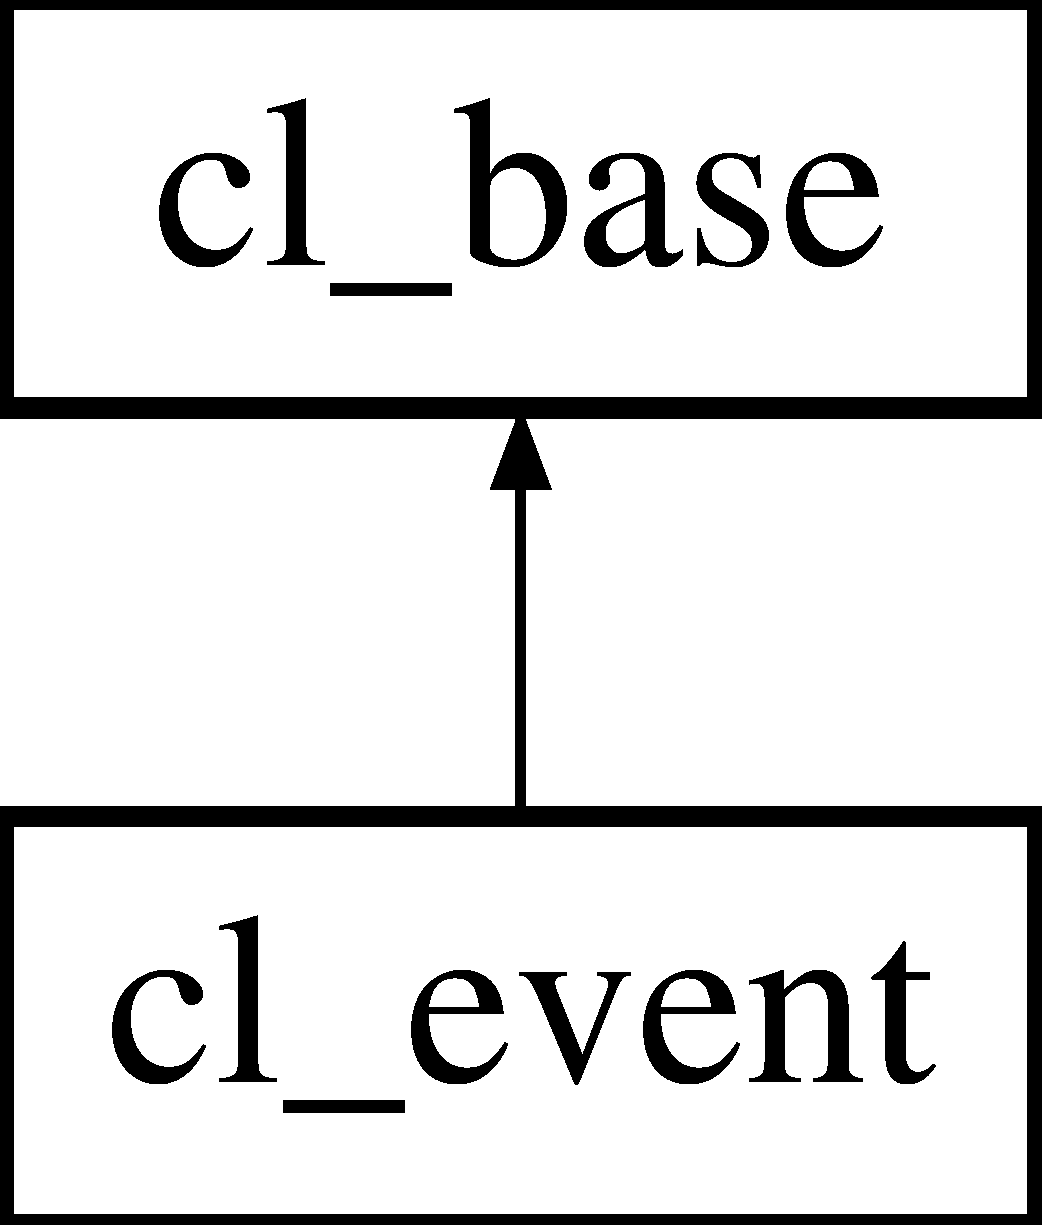
\includegraphics[height=2.000000cm]{classcl__event}
\end{center}
\end{figure}
\subsection*{Public Member Functions}
\begin{DoxyCompactItemize}
\item 
\hypertarget{classcl__event_a51feb0f638fed8930a604a648b6245c6}{
{\bfseries cl\_\-event} (enum event what\_\-event)}
\label{classcl__event_a51feb0f638fed8930a604a648b6245c6}

\item 
\hypertarget{classcl__event_aadc059c23d68bae87ca2877d79cb07df}{
bool {\bfseries is\_\-handled} (void)}
\label{classcl__event_aadc059c23d68bae87ca2877d79cb07df}

\item 
\hypertarget{classcl__event_a49d88839722b9ae1923291685bd2409a}{
virtual void {\bfseries handle} (void)}
\label{classcl__event_a49d88839722b9ae1923291685bd2409a}

\end{DoxyCompactItemize}
\subsection*{Public Attributes}
\begin{DoxyCompactItemize}
\item 
\hypertarget{classcl__event_a1c24ef7077a204036b71cf57f12f2b36}{
enum event {\bfseries what}}
\label{classcl__event_a1c24ef7077a204036b71cf57f12f2b36}

\end{DoxyCompactItemize}
\subsection*{Protected Attributes}
\begin{DoxyCompactItemize}
\item 
\hypertarget{classcl__event_ad3d054e066f076207569b3f3151b1a23}{
bool {\bfseries handled}}
\label{classcl__event_ad3d054e066f076207569b3f3151b1a23}

\end{DoxyCompactItemize}


The documentation for this class was generated from the following files:\begin{DoxyCompactItemize}
\item 
pobjcl.h\item 
pobj.cc\end{DoxyCompactItemize}

\hypertarget{classcl__float__option}{
\section{cl\_\-float\_\-option Class Reference}
\label{classcl__float__option}\index{cl\_\-float\_\-option@{cl\_\-float\_\-option}}
}
Inheritance diagram for cl\_\-float\_\-option:\begin{figure}[H]
\begin{center}
\leavevmode
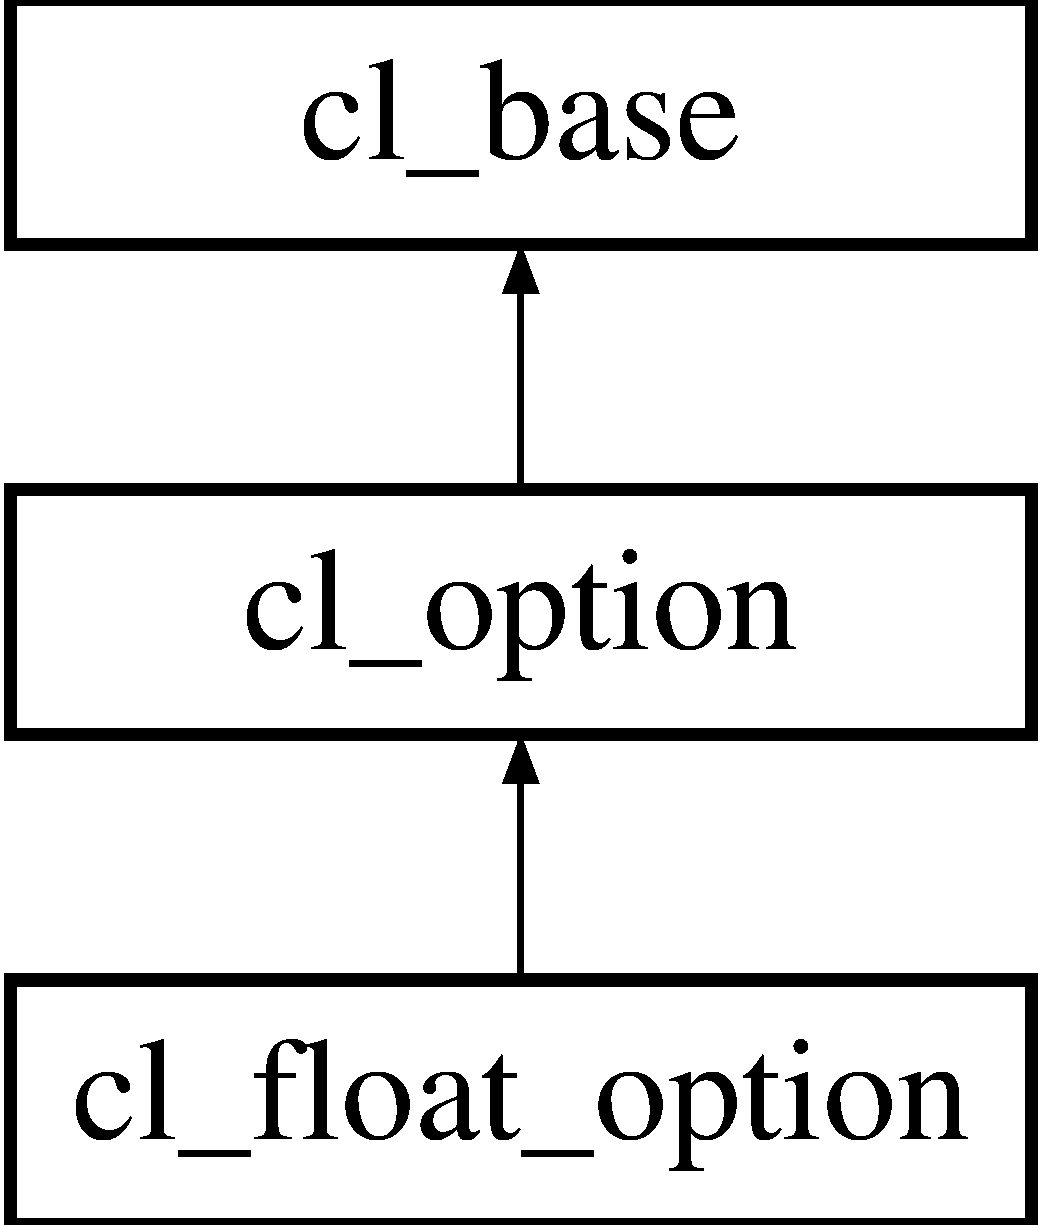
\includegraphics[height=3.000000cm]{classcl__float__option}
\end{center}
\end{figure}
\subsection*{Public Member Functions}
\begin{DoxyCompactItemize}
\item 
\hypertarget{classcl__float__option_a097eb653d4d6b14ff488467de9bb06a4}{
{\bfseries cl\_\-float\_\-option} (class \hyperlink{classcl__base}{cl\_\-base} $\ast$the\_\-creator, char $\ast$aname, char $\ast$Ihelp)}
\label{classcl__float__option_a097eb653d4d6b14ff488467de9bb06a4}

\item 
\hypertarget{classcl__float__option_a9c3c7793d5fe36c996340855cb6af6cc}{
virtual void {\bfseries print} (class cl\_\-console $\ast$con)}
\label{classcl__float__option_a9c3c7793d5fe36c996340855cb6af6cc}

\item 
\hypertarget{classcl__float__option_ac469d0cd98a4aedcb2eabdf7d84e577e}{
virtual char $\ast$ {\bfseries get\_\-type\_\-name} (void)}
\label{classcl__float__option_ac469d0cd98a4aedcb2eabdf7d84e577e}

\item 
\hypertarget{classcl__float__option_a3a0677e34a43913f3796d977a8bf67c3}{
virtual void {\bfseries set\_\-value} (char $\ast$s)}
\label{classcl__float__option_a3a0677e34a43913f3796d977a8bf67c3}

\end{DoxyCompactItemize}


The documentation for this class was generated from the following files:\begin{DoxyCompactItemize}
\item 
optioncl.h\item 
option.cc\end{DoxyCompactItemize}

\hypertarget{classcl__list}{
\section{cl\_\-list Class Reference}
\label{classcl__list}\index{cl\_\-list@{cl\_\-list}}
}
Inheritance diagram for cl\_\-list:\begin{figure}[H]
\begin{center}
\leavevmode
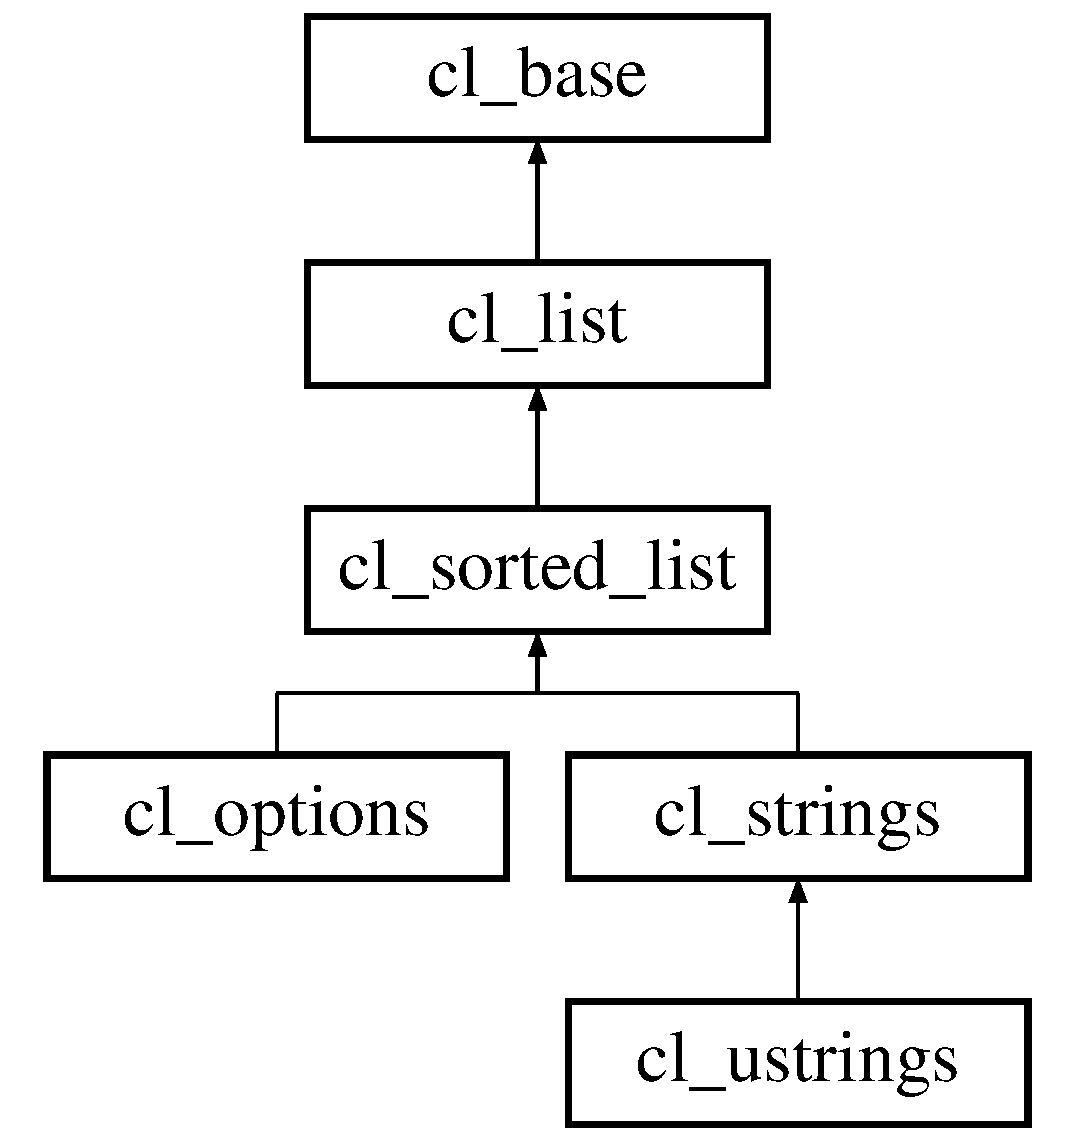
\includegraphics[height=5.000000cm]{classcl__list}
\end{center}
\end{figure}
\subsection*{Public Member Functions}
\begin{DoxyCompactItemize}
\item 
\hypertarget{classcl__list_a85d92f26e22d8ad00416ad7e26e85409}{
{\bfseries cl\_\-list} (t\_\-index alimit, t\_\-index adelta, char $\ast$aname)}
\label{classcl__list_a85d92f26e22d8ad00416ad7e26e85409}

\item 
\hypertarget{classcl__list_ac7d6177ed937048bfd5fc673b618d89a}{
void $\ast$ {\bfseries at} (t\_\-index index)}
\label{classcl__list_ac7d6177ed937048bfd5fc673b618d89a}

\item 
\hypertarget{classcl__list_a750c847d848f93c55acebb27336bde32}{
class \hyperlink{classcl__base}{cl\_\-base} $\ast$ {\bfseries object\_\-at} (t\_\-index index)}
\label{classcl__list_a750c847d848f93c55acebb27336bde32}

\item 
\hypertarget{classcl__list_a2e410f26d12453d1699ea2c808e506b7}{
virtual t\_\-index {\bfseries index\_\-of} (void $\ast$item)}
\label{classcl__list_a2e410f26d12453d1699ea2c808e506b7}

\item 
\hypertarget{classcl__list_a7eae53736d6028803aaf2fea5188d1e5}{
virtual bool {\bfseries index\_\-of} (void $\ast$item, t\_\-index $\ast$idx)}
\label{classcl__list_a7eae53736d6028803aaf2fea5188d1e5}

\item 
\hypertarget{classcl__list_aef0456132d8b16abbb82ea88d272ddb7}{
virtual void $\ast$ {\bfseries next} (void $\ast$item)}
\label{classcl__list_aef0456132d8b16abbb82ea88d272ddb7}

\item 
\hypertarget{classcl__list_a538c92d61f98cc76d751bff1b9464a97}{
int {\bfseries get\_\-count} (void)}
\label{classcl__list_a538c92d61f98cc76d751bff1b9464a97}

\item 
\hypertarget{classcl__list_a1e67e4531eecd5f51673f9c6d1ada13a}{
virtual void $\ast$ {\bfseries pop} (void)}
\label{classcl__list_a1e67e4531eecd5f51673f9c6d1ada13a}

\item 
\hypertarget{classcl__list_ae5518c248f803c95a9395e205f4bbc5e}{
virtual void $\ast$ {\bfseries top} (void)}
\label{classcl__list_ae5518c248f803c95a9395e205f4bbc5e}

\item 
\hypertarget{classcl__list_ae233fbd20ae5ccdda7a0375eadb3b5d3}{
virtual void {\bfseries set\_\-limit} (t\_\-index alimit)}
\label{classcl__list_ae233fbd20ae5ccdda7a0375eadb3b5d3}

\item 
\hypertarget{classcl__list_ae738dd14c8f67f800d7c06bc723171f8}{
void {\bfseries free\_\-at} (t\_\-index index)}
\label{classcl__list_ae738dd14c8f67f800d7c06bc723171f8}

\item 
\hypertarget{classcl__list_ac992d70be5612e3a251d00ccae8db9b6}{
void {\bfseries free\_\-all} (void)}
\label{classcl__list_ac992d70be5612e3a251d00ccae8db9b6}

\item 
\hypertarget{classcl__list_a10444fbbd9e9379b055ccbdb0f1d48e7}{
void {\bfseries disconn\_\-at} (t\_\-index index)}
\label{classcl__list_a10444fbbd9e9379b055ccbdb0f1d48e7}

\item 
\hypertarget{classcl__list_a133204c93e910354549192660220225f}{
void {\bfseries disconn} (void $\ast$item)}
\label{classcl__list_a133204c93e910354549192660220225f}

\item 
\hypertarget{classcl__list_a0ae50538730bdca29fc2d4fbaf086274}{
void {\bfseries disconn\_\-all} (void)}
\label{classcl__list_a0ae50538730bdca29fc2d4fbaf086274}

\item 
\hypertarget{classcl__list_af29ad14994376973e07be4246d42043e}{
void {\bfseries add\_\-at} (t\_\-index index, void $\ast$item)}
\label{classcl__list_af29ad14994376973e07be4246d42043e}

\item 
\hypertarget{classcl__list_a49e7f12ec480a37415f4d7b84a6e4051}{
void {\bfseries put\_\-at} (t\_\-index index, void $\ast$item)}
\label{classcl__list_a49e7f12ec480a37415f4d7b84a6e4051}

\item 
\hypertarget{classcl__list_a562ab977d9cc496e10af548b06142f73}{
virtual t\_\-index {\bfseries add} (void $\ast$item)}
\label{classcl__list_a562ab977d9cc496e10af548b06142f73}

\item 
\hypertarget{classcl__list_a9fa74743220cae9203747bd719b243a6}{
virtual t\_\-index {\bfseries add} (class \hyperlink{classcl__base}{cl\_\-base} $\ast$item, class \hyperlink{classcl__base}{cl\_\-base} $\ast$parent)}
\label{classcl__list_a9fa74743220cae9203747bd719b243a6}

\item 
\hypertarget{classcl__list_ad23d1c54162dd0249295290a7eded4fc}{
virtual void {\bfseries push} (void $\ast$item)}
\label{classcl__list_ad23d1c54162dd0249295290a7eded4fc}

\item 
\hypertarget{classcl__list_a48be20e7bb978fb86af3b15d332a0779}{
void $\ast$ {\bfseries first\_\-that} (match\_\-func test, void $\ast$arg)}
\label{classcl__list_a48be20e7bb978fb86af3b15d332a0779}

\item 
\hypertarget{classcl__list_afd2e651e8ee471d31c0ca5466cf17caa}{
void $\ast$ {\bfseries last\_\-that} (match\_\-func test, void $\ast$arg)}
\label{classcl__list_afd2e651e8ee471d31c0ca5466cf17caa}

\item 
\hypertarget{classcl__list_ac4d0073073329fac159aa6908450984a}{
void {\bfseries for\_\-each} (iterator\_\-func action, void $\ast$arg)}
\label{classcl__list_ac4d0073073329fac159aa6908450984a}

\item 
\hypertarget{classcl__list_acf5777e046c1c0f1ea433e4998422f46}{
void {\bfseries error} (t\_\-index code, t\_\-index info)}
\label{classcl__list_acf5777e046c1c0f1ea433e4998422f46}

\end{DoxyCompactItemize}
\subsection*{Public Attributes}
\begin{DoxyCompactItemize}
\item 
\hypertarget{classcl__list_af6b118ba286729469cface6d412a53c3}{
t\_\-index {\bfseries count}}
\label{classcl__list_af6b118ba286729469cface6d412a53c3}

\end{DoxyCompactItemize}
\subsection*{Protected Attributes}
\begin{DoxyCompactItemize}
\item 
\hypertarget{classcl__list_a793ad4228dd48d1ea1dd6b08319b5870}{
void $\ast$$\ast$ {\bfseries Items}}
\label{classcl__list_a793ad4228dd48d1ea1dd6b08319b5870}

\item 
\hypertarget{classcl__list_a40bcb89ac023574fd389cb30664b664b}{
t\_\-index {\bfseries Limit}}
\label{classcl__list_a40bcb89ac023574fd389cb30664b664b}

\item 
\hypertarget{classcl__list_ab896ba4e70d00406bcdbcbea0d5f1c05}{
t\_\-index {\bfseries Delta}}
\label{classcl__list_ab896ba4e70d00406bcdbcbea0d5f1c05}

\end{DoxyCompactItemize}


The documentation for this class was generated from the following files:\begin{DoxyCompactItemize}
\item 
pobjcl.h\item 
pobj.cc\end{DoxyCompactItemize}

\hypertarget{classcl__number__option}{
\section{cl\_\-number\_\-option Class Reference}
\label{classcl__number__option}\index{cl\_\-number\_\-option@{cl\_\-number\_\-option}}
}
Inheritance diagram for cl\_\-number\_\-option:\begin{figure}[H]
\begin{center}
\leavevmode
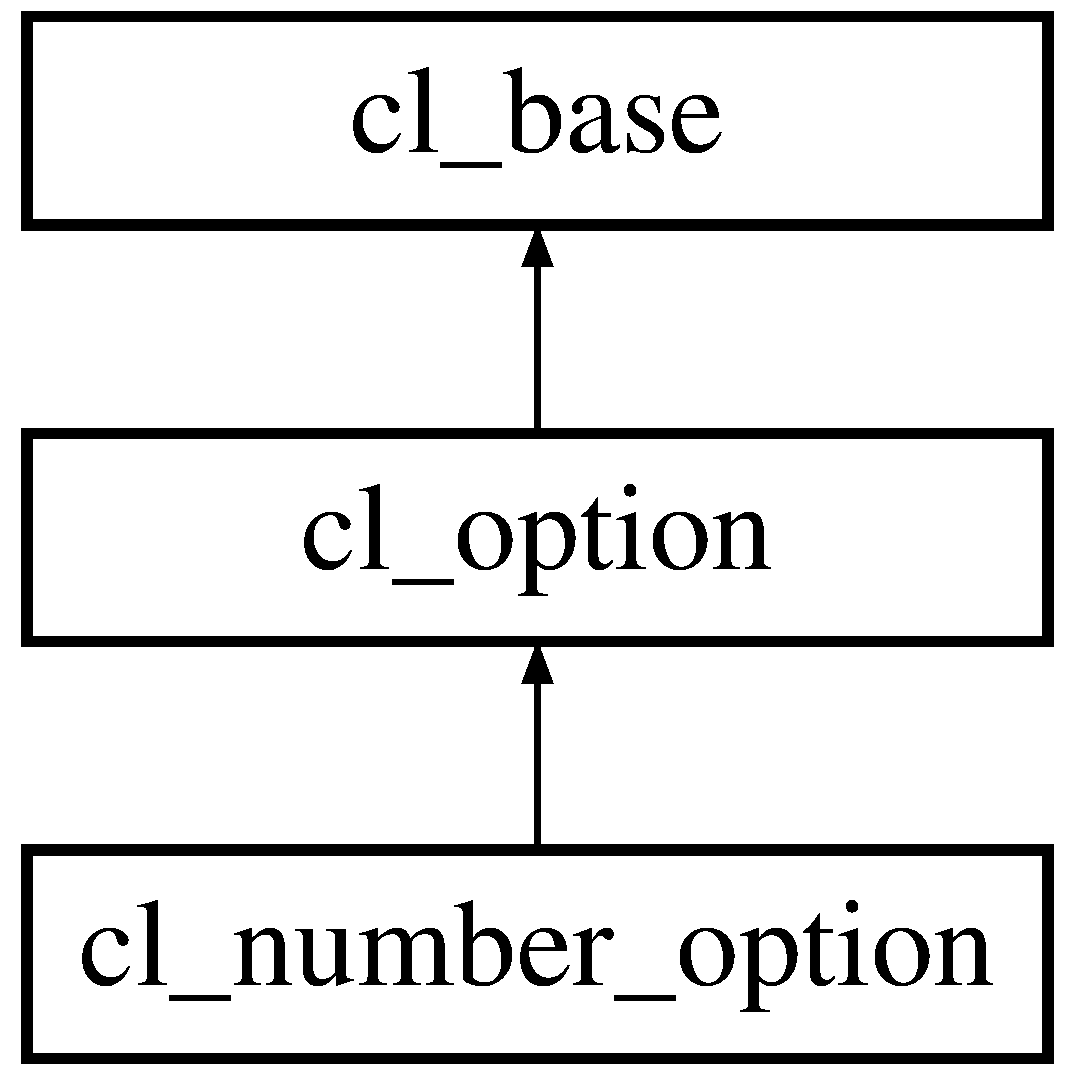
\includegraphics[height=3.000000cm]{classcl__number__option}
\end{center}
\end{figure}
\subsection*{Public Member Functions}
\begin{DoxyCompactItemize}
\item 
\hypertarget{classcl__number__option_abe01b67a88d03bd49b3b7f8057e68c8e}{
{\bfseries cl\_\-number\_\-option} (class \hyperlink{classcl__base}{cl\_\-base} $\ast$the\_\-creator, char $\ast$aname, char $\ast$Ihelp)}
\label{classcl__number__option_abe01b67a88d03bd49b3b7f8057e68c8e}

\item 
\hypertarget{classcl__number__option_a8e5f72c9f87729e2532589f076dffe28}{
virtual void {\bfseries print} (class cl\_\-console $\ast$con)}
\label{classcl__number__option_a8e5f72c9f87729e2532589f076dffe28}

\item 
\hypertarget{classcl__number__option_a158af3f1fee1a1f9acffa9eb1a1a4b3b}{
virtual char $\ast$ {\bfseries get\_\-type\_\-name} (void)}
\label{classcl__number__option_a158af3f1fee1a1f9acffa9eb1a1a4b3b}

\item 
\hypertarget{classcl__number__option_a4c3464a6b48f0d6daa547bcba3b15402}{
virtual void {\bfseries set\_\-value} (char $\ast$s)}
\label{classcl__number__option_a4c3464a6b48f0d6daa547bcba3b15402}

\end{DoxyCompactItemize}


The documentation for this class was generated from the following files:\begin{DoxyCompactItemize}
\item 
optioncl.h\item 
option.cc\end{DoxyCompactItemize}

\hypertarget{classcl__option}{
\section{cl\_\-option Class Reference}
\label{classcl__option}\index{cl\_\-option@{cl\_\-option}}
}
Inheritance diagram for cl\_\-option:\begin{figure}[H]
\begin{center}
\leavevmode
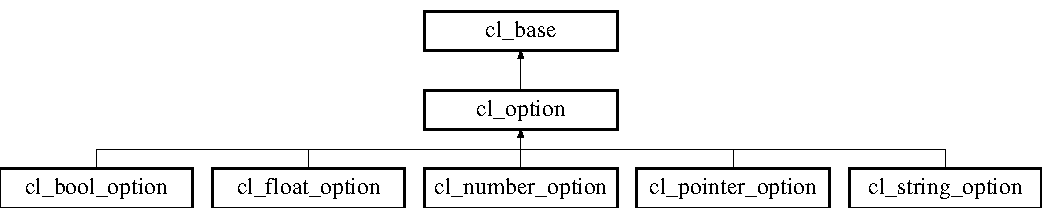
\includegraphics[height=2.800000cm]{classcl__option}
\end{center}
\end{figure}
\subsection*{Public Member Functions}
\begin{DoxyCompactItemize}
\item 
\hypertarget{classcl__option_a52aee9817e2fe084379419f204d8d660}{
{\bfseries cl\_\-option} (class \hyperlink{classcl__base}{cl\_\-base} $\ast$the\_\-creator, char $\ast$aname, char $\ast$Ihelp)}
\label{classcl__option_a52aee9817e2fe084379419f204d8d660}

\item 
\hypertarget{classcl__option_a974b7e378703a036c393e569cfbf093a}{
virtual class \hyperlink{classcl__option}{cl\_\-option} \& {\bfseries operator=} (class \hyperlink{classcl__option}{cl\_\-option} \&o)}
\label{classcl__option_a974b7e378703a036c393e569cfbf093a}

\item 
\hypertarget{classcl__option_a50496fdfcf2615d97374bc45084e2679}{
virtual void {\bfseries pre\_\-remove} (void)}
\label{classcl__option_a50496fdfcf2615d97374bc45084e2679}

\item 
\hypertarget{classcl__option_ac2ce92605135b725ca7167968832d69f}{
virtual class \hyperlink{classcl__base}{cl\_\-base} $\ast$ {\bfseries get\_\-creator} (void)}
\label{classcl__option_ac2ce92605135b725ca7167968832d69f}

\item 
\hypertarget{classcl__option_a9666c5ad17c176456e3768ede3fe37e9}{
virtual void {\bfseries hide} (void)}
\label{classcl__option_a9666c5ad17c176456e3768ede3fe37e9}

\item 
\hypertarget{classcl__option_ace1e7456180a339b220bb0b09128d694}{
virtual void {\bfseries show} (void)}
\label{classcl__option_ace1e7456180a339b220bb0b09128d694}

\item 
\hypertarget{classcl__option_a357c40dde81a6331c48933e558c5bc57}{
virtual void {\bfseries print} (class cl\_\-console $\ast$con)}
\label{classcl__option_a357c40dde81a6331c48933e558c5bc57}

\item 
\hypertarget{classcl__option_a23a99f00e80e4155cf11e7e6ba4cbc4b}{
virtual char $\ast$ {\bfseries get\_\-type\_\-name} (void)}
\label{classcl__option_a23a99f00e80e4155cf11e7e6ba4cbc4b}

\item 
\hypertarget{classcl__option_a3bc048ec1d4a2b984f6e9adfce35f197}{
virtual union \hyperlink{unionoption__value}{option\_\-value} $\ast$ {\bfseries get\_\-value} (void)}
\label{classcl__option_a3bc048ec1d4a2b984f6e9adfce35f197}

\item 
\hypertarget{classcl__option_a82a7db3689075194c0d7a78f25e3f225}{
virtual void {\bfseries get\_\-value} (bool $\ast$val)}
\label{classcl__option_a82a7db3689075194c0d7a78f25e3f225}

\item 
\hypertarget{classcl__option_adb46012b2855f29c4db42836bd22daa6}{
virtual void {\bfseries get\_\-value} (char $\ast$$\ast$val)}
\label{classcl__option_adb46012b2855f29c4db42836bd22daa6}

\item 
\hypertarget{classcl__option_afa0b7f7eaaa194b14ee9582ec18b8919}{
virtual void {\bfseries get\_\-value} (void $\ast$$\ast$val)}
\label{classcl__option_afa0b7f7eaaa194b14ee9582ec18b8919}

\item 
\hypertarget{classcl__option_a3c982c06a85d7f2432a37fc0fe574461}{
virtual void {\bfseries get\_\-value} (long $\ast$val)}
\label{classcl__option_a3c982c06a85d7f2432a37fc0fe574461}

\item 
\hypertarget{classcl__option_a84c3a129fe6a5ed5993f39773309b822}{
virtual void {\bfseries get\_\-value} (double $\ast$val)}
\label{classcl__option_a84c3a129fe6a5ed5993f39773309b822}

\item 
\hypertarget{classcl__option_af3f92c6bf942c17d85b72f784e540f86}{
virtual void {\bfseries set\_\-value} (bool opt)}
\label{classcl__option_af3f92c6bf942c17d85b72f784e540f86}

\item 
\hypertarget{classcl__option_ad99fa2f47bf6cda998eeb6c6129cc58d}{
virtual void {\bfseries set\_\-value} (char $\ast$opt)}
\label{classcl__option_ad99fa2f47bf6cda998eeb6c6129cc58d}

\item 
\hypertarget{classcl__option_a22c98f85b7277e32a381290eb93956b4}{
virtual void {\bfseries set\_\-value} (void $\ast$opt)}
\label{classcl__option_a22c98f85b7277e32a381290eb93956b4}

\item 
\hypertarget{classcl__option_a5cffed6fbd8627ac67f59ec666b429f5}{
virtual void {\bfseries set\_\-value} (long opt)}
\label{classcl__option_a5cffed6fbd8627ac67f59ec666b429f5}

\item 
\hypertarget{classcl__option_adbfbcb7cdd32dd03747788847c61b928}{
virtual void {\bfseries set\_\-value} (double opt)}
\label{classcl__option_adbfbcb7cdd32dd03747788847c61b928}

\item 
\hypertarget{classcl__option_abda5402689da9bdfaf7a4292e79a3794}{
virtual void {\bfseries new\_\-reference} (class \hyperlink{classcl__optref}{cl\_\-optref} $\ast$ref)}
\label{classcl__option_abda5402689da9bdfaf7a4292e79a3794}

\item 
\hypertarget{classcl__option_a171748b865f73e9f84918795a1a5c109}{
virtual void {\bfseries del\_\-reference} (class \hyperlink{classcl__optref}{cl\_\-optref} $\ast$ref)}
\label{classcl__option_a171748b865f73e9f84918795a1a5c109}

\item 
\hypertarget{classcl__option_a745397439967699a9fc8814b39361a77}{
virtual void {\bfseries inform\_\-users} (void)}
\label{classcl__option_a745397439967699a9fc8814b39361a77}

\end{DoxyCompactItemize}
\subsection*{Public Attributes}
\begin{DoxyCompactItemize}
\item 
\hypertarget{classcl__option_a1483c8dd62e5992e7b4e5577f257bf5c}{
class \hyperlink{classcl__list}{cl\_\-list} $\ast$ {\bfseries users}}
\label{classcl__option_a1483c8dd62e5992e7b4e5577f257bf5c}

\item 
\hypertarget{classcl__option_a4af07a7cc992a83e6108b11acfc6e4ce}{
char $\ast$ {\bfseries help}}
\label{classcl__option_a4af07a7cc992a83e6108b11acfc6e4ce}

\item 
\hypertarget{classcl__option_ad71d5473e16cbebacab79220ea0349b7}{
bool {\bfseries hidden}}
\label{classcl__option_ad71d5473e16cbebacab79220ea0349b7}

\end{DoxyCompactItemize}
\subsection*{Protected Attributes}
\begin{DoxyCompactItemize}
\item 
\hypertarget{classcl__option_acbb8db0fe549d278c38290d357aaace5}{
void $\ast$ {\bfseries option}}
\label{classcl__option_acbb8db0fe549d278c38290d357aaace5}

\item 
\hypertarget{classcl__option_a0aed4ba999857ebb65589e214484f198}{
union \hyperlink{unionoption__value}{option\_\-value} {\bfseries value}}
\label{classcl__option_a0aed4ba999857ebb65589e214484f198}

\item 
\hypertarget{classcl__option_a3ae9fa397a3665941b1af35650d2a24a}{
class \hyperlink{classcl__base}{cl\_\-base} $\ast$ {\bfseries creator}}
\label{classcl__option_a3ae9fa397a3665941b1af35650d2a24a}

\end{DoxyCompactItemize}


The documentation for this class was generated from the following files:\begin{DoxyCompactItemize}
\item 
optioncl.h\item 
option.cc\end{DoxyCompactItemize}

\hypertarget{classcl__options}{
\section{cl\_\-options Class Reference}
\label{classcl__options}\index{cl\_\-options@{cl\_\-options}}
}
Inheritance diagram for cl\_\-options:\begin{figure}[H]
\begin{center}
\leavevmode
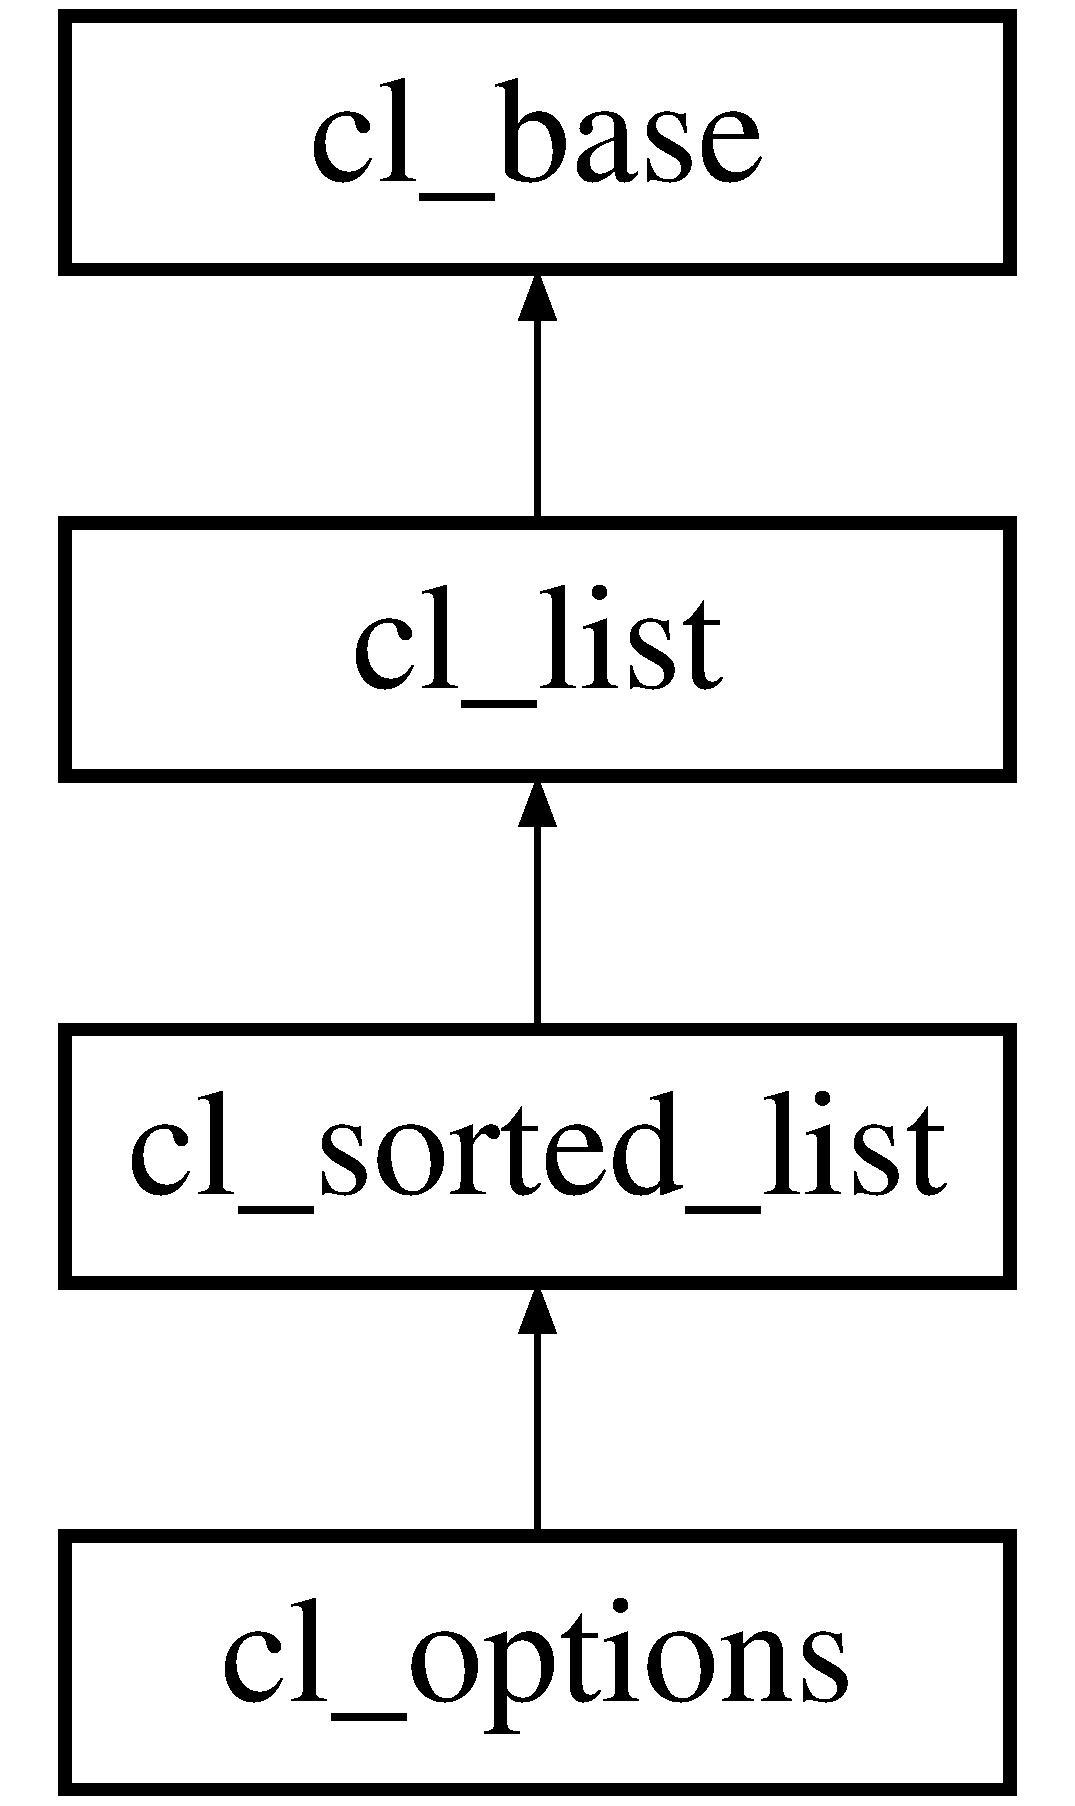
\includegraphics[height=4.000000cm]{classcl__options}
\end{center}
\end{figure}
\subsection*{Public Member Functions}
\begin{DoxyCompactItemize}
\item 
\hypertarget{classcl__options_afe9b229be92e3ddc519602cbafb087dc}{
virtual void $\ast$ {\bfseries key\_\-of} (void $\ast$item)}
\label{classcl__options_afe9b229be92e3ddc519602cbafb087dc}

\item 
\hypertarget{classcl__options_a30e9265492e08c86ebd15d032ba53cb5}{
virtual int {\bfseries compare} (void $\ast$key1, void $\ast$key2)}
\label{classcl__options_a30e9265492e08c86ebd15d032ba53cb5}

\item 
\hypertarget{classcl__options_a558bbdd448f06b5055c83c40400bb0b1}{
virtual void {\bfseries new\_\-option} (class \hyperlink{classcl__option}{cl\_\-option} $\ast$opt)}
\label{classcl__options_a558bbdd448f06b5055c83c40400bb0b1}

\item 
\hypertarget{classcl__options_acfd2a6d1424056903ce6c945f46871e8}{
virtual void {\bfseries del\_\-option} (class \hyperlink{classcl__option}{cl\_\-option} $\ast$opt)}
\label{classcl__options_acfd2a6d1424056903ce6c945f46871e8}

\item 
\hypertarget{classcl__options_a27b0bf51c5657f9ac8fa2acb2ec79ff2}{
virtual class \hyperlink{classcl__option}{cl\_\-option} $\ast$ {\bfseries get\_\-option} (char $\ast$the\_\-name)}
\label{classcl__options_a27b0bf51c5657f9ac8fa2acb2ec79ff2}

\item 
\hypertarget{classcl__options_ab7683f05307308b4f676474c3f547955}{
virtual class \hyperlink{classcl__option}{cl\_\-option} $\ast$ {\bfseries get\_\-option} (char $\ast$the\_\-name, class \hyperlink{classcl__base}{cl\_\-base} $\ast$creator)}
\label{classcl__options_ab7683f05307308b4f676474c3f547955}

\item 
\hypertarget{classcl__options_aebf3d2761d774685c51bf7e8de5d2f25}{
virtual class \hyperlink{classcl__option}{cl\_\-option} $\ast$ {\bfseries get\_\-option} (char $\ast$the\_\-name, char $\ast$creator)}
\label{classcl__options_aebf3d2761d774685c51bf7e8de5d2f25}

\item 
\hypertarget{classcl__options_a989e623395c0f7e3e9593db236380045}{
virtual class \hyperlink{classcl__option}{cl\_\-option} $\ast$ {\bfseries get\_\-option} (int idx)}
\label{classcl__options_a989e623395c0f7e3e9593db236380045}

\item 
\hypertarget{classcl__options_a0a495dafa4dae61dbcd14335d1b510b9}{
virtual int {\bfseries nuof\_\-options} (char $\ast$the\_\-name)}
\label{classcl__options_a0a495dafa4dae61dbcd14335d1b510b9}

\item 
\hypertarget{classcl__options_a2549d33961d9fbc55a3dcd87c4b51bf6}{
virtual int {\bfseries nuof\_\-options} (char $\ast$the\_\-name, char $\ast$creator)}
\label{classcl__options_a2549d33961d9fbc55a3dcd87c4b51bf6}

\item 
\hypertarget{classcl__options_a8f1b5df5a74df3a2f5486ba2a674da81}{
virtual class \hyperlink{classcl__option}{cl\_\-option} $\ast$ {\bfseries set\_\-value} (char $\ast$the\_\-name, \hyperlink{classcl__base}{cl\_\-base} $\ast$creator, bool value)}
\label{classcl__options_a8f1b5df5a74df3a2f5486ba2a674da81}

\item 
\hypertarget{classcl__options_a97789e2ce959ab98414627429452f899}{
virtual class \hyperlink{classcl__option}{cl\_\-option} $\ast$ {\bfseries set\_\-value} (char $\ast$the\_\-name, \hyperlink{classcl__base}{cl\_\-base} $\ast$creator, char $\ast$value)}
\label{classcl__options_a97789e2ce959ab98414627429452f899}

\item 
\hypertarget{classcl__options_a2d6a1f000cbe666ffb36e57e0795b743}{
virtual class \hyperlink{classcl__option}{cl\_\-option} $\ast$ {\bfseries set\_\-value} (char $\ast$the\_\-name, \hyperlink{classcl__base}{cl\_\-base} $\ast$creator, void $\ast$value)}
\label{classcl__options_a2d6a1f000cbe666ffb36e57e0795b743}

\item 
\hypertarget{classcl__options_ad8f398ba46e39ef8995642b0d2da4ab9}{
virtual class \hyperlink{classcl__option}{cl\_\-option} $\ast$ {\bfseries set\_\-value} (char $\ast$the\_\-name, \hyperlink{classcl__base}{cl\_\-base} $\ast$creator, long value)}
\label{classcl__options_ad8f398ba46e39ef8995642b0d2da4ab9}

\item 
\hypertarget{classcl__options_a5df4aef619ea72a8acc63aff30353776}{
virtual class \hyperlink{classcl__option}{cl\_\-option} $\ast$ {\bfseries set\_\-value} (char $\ast$the\_\-name, \hyperlink{classcl__base}{cl\_\-base} $\ast$creator, double value)}
\label{classcl__options_a5df4aef619ea72a8acc63aff30353776}

\end{DoxyCompactItemize}


The documentation for this class was generated from the following files:\begin{DoxyCompactItemize}
\item 
optioncl.h\item 
option.cc\end{DoxyCompactItemize}

\hypertarget{classcl__optref}{
\section{cl\_\-optref Class Reference}
\label{classcl__optref}\index{cl\_\-optref@{cl\_\-optref}}
}
Inheritance diagram for cl\_\-optref:\begin{figure}[H]
\begin{center}
\leavevmode
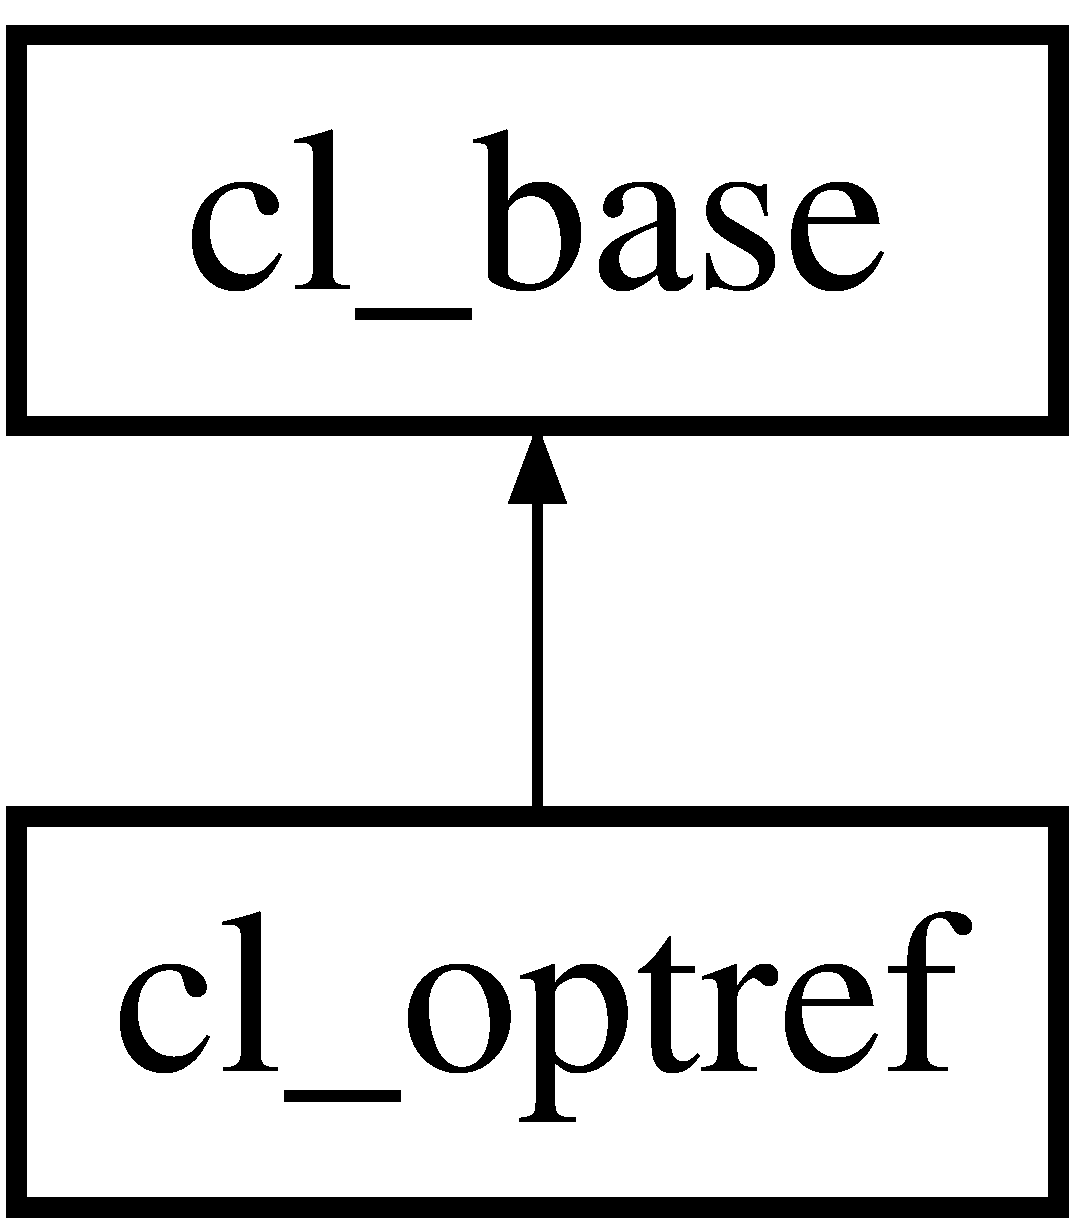
\includegraphics[height=2.000000cm]{classcl__optref}
\end{center}
\end{figure}
\subsection*{Public Member Functions}
\begin{DoxyCompactItemize}
\item 
\hypertarget{classcl__optref_ab7c07bbe5705316a9c23ec7c38e9c975}{
{\bfseries cl\_\-optref} (class \hyperlink{classcl__base}{cl\_\-base} $\ast$the\_\-owner)}
\label{classcl__optref_ab7c07bbe5705316a9c23ec7c38e9c975}

\item 
\hypertarget{classcl__optref_a24843e8bfc2b8db98538764339352b83}{
{\bfseries cl\_\-optref} (class \hyperlink{classcl__base}{cl\_\-base} $\ast$the\_\-owner, class \hyperlink{classcl__option}{cl\_\-option} $\ast$new\_\-option)}
\label{classcl__optref_a24843e8bfc2b8db98538764339352b83}

\item 
\hypertarget{classcl__optref_a8b46fe1d6e839680848460556882a6c2}{
virtual class \hyperlink{classcl__option}{cl\_\-option} $\ast$ {\bfseries create} (class \hyperlink{classcl__base}{cl\_\-base} $\ast$creator, enum option\_\-type type, char $\ast$the\_\-name, char $\ast$help)}
\label{classcl__optref_a8b46fe1d6e839680848460556882a6c2}

\item 
\hypertarget{classcl__optref_a0a6b5e02bd6f3e6d569525c48ad43c99}{
virtual void {\bfseries default\_\-option} (char $\ast$the\_\-name)}
\label{classcl__optref_a0a6b5e02bd6f3e6d569525c48ad43c99}

\item 
\hypertarget{classcl__optref_a221904bbfb3a18b9c7b5d4deb23b7337}{
virtual class \hyperlink{classcl__option}{cl\_\-option} $\ast$ {\bfseries use} (void)}
\label{classcl__optref_a221904bbfb3a18b9c7b5d4deb23b7337}

\item 
\hypertarget{classcl__optref_a7843e9587f17606c09dfe0939bc11a35}{
virtual class \hyperlink{classcl__option}{cl\_\-option} $\ast$ {\bfseries use} (char $\ast$the\_\-name)}
\label{classcl__optref_a7843e9587f17606c09dfe0939bc11a35}

\item 
\hypertarget{classcl__optref_a802b37c29ec2d274830269a1c372ca5a}{
virtual void {\bfseries option\_\-changed} (void)}
\label{classcl__optref_a802b37c29ec2d274830269a1c372ca5a}

\item 
\hypertarget{classcl__optref_aff9dba037ce41ea6afb578635c528335}{
virtual void {\bfseries option\_\-removing} (void)}
\label{classcl__optref_aff9dba037ce41ea6afb578635c528335}

\item 
\hypertarget{classcl__optref_a281ae14ca1cff9bb1e8cc61ded245dec}{
virtual class \hyperlink{classcl__base}{cl\_\-base} $\ast$ {\bfseries get\_\-owner} (void)}
\label{classcl__optref_a281ae14ca1cff9bb1e8cc61ded245dec}

\item 
\hypertarget{classcl__optref_a0794160f2fa675366c6ee88f9136875f}{
virtual bool {\bfseries get\_\-value} (bool)}
\label{classcl__optref_a0794160f2fa675366c6ee88f9136875f}

\item 
\hypertarget{classcl__optref_a0ad86a93d20f82905b63f2ec81f50961}{
virtual char $\ast$ {\bfseries get\_\-value} (char $\ast$)}
\label{classcl__optref_a0ad86a93d20f82905b63f2ec81f50961}

\item 
\hypertarget{classcl__optref_a1ff9c3b5605ef99451515e495b4b785a}{
virtual void $\ast$ {\bfseries get\_\-value} (void $\ast$)}
\label{classcl__optref_a1ff9c3b5605ef99451515e495b4b785a}

\item 
\hypertarget{classcl__optref_a1e9567c9088f7fa9d98e5d3484ce77b1}{
virtual long {\bfseries get\_\-value} (long)}
\label{classcl__optref_a1e9567c9088f7fa9d98e5d3484ce77b1}

\item 
\hypertarget{classcl__optref_af11f6cc27f00273fedf01122843deb80}{
virtual double {\bfseries get\_\-value} (double)}
\label{classcl__optref_af11f6cc27f00273fedf01122843deb80}

\end{DoxyCompactItemize}
\subsection*{Protected Attributes}
\begin{DoxyCompactItemize}
\item 
\hypertarget{classcl__optref_a9234d980ec032f48dd137ed2676eb815}{
class \hyperlink{classcl__option}{cl\_\-option} $\ast$ {\bfseries option}}
\label{classcl__optref_a9234d980ec032f48dd137ed2676eb815}

\item 
\hypertarget{classcl__optref_a483428efce1211af9ba5e51296257820}{
class \hyperlink{classcl__base}{cl\_\-base} $\ast$ {\bfseries owner}}
\label{classcl__optref_a483428efce1211af9ba5e51296257820}

\end{DoxyCompactItemize}


The documentation for this class was generated from the following files:\begin{DoxyCompactItemize}
\item 
optioncl.h\item 
option.cc\end{DoxyCompactItemize}

\hypertarget{classcl__pointer__option}{
\section{cl\_\-pointer\_\-option Class Reference}
\label{classcl__pointer__option}\index{cl\_\-pointer\_\-option@{cl\_\-pointer\_\-option}}
}
Inheritance diagram for cl\_\-pointer\_\-option:\begin{figure}[H]
\begin{center}
\leavevmode
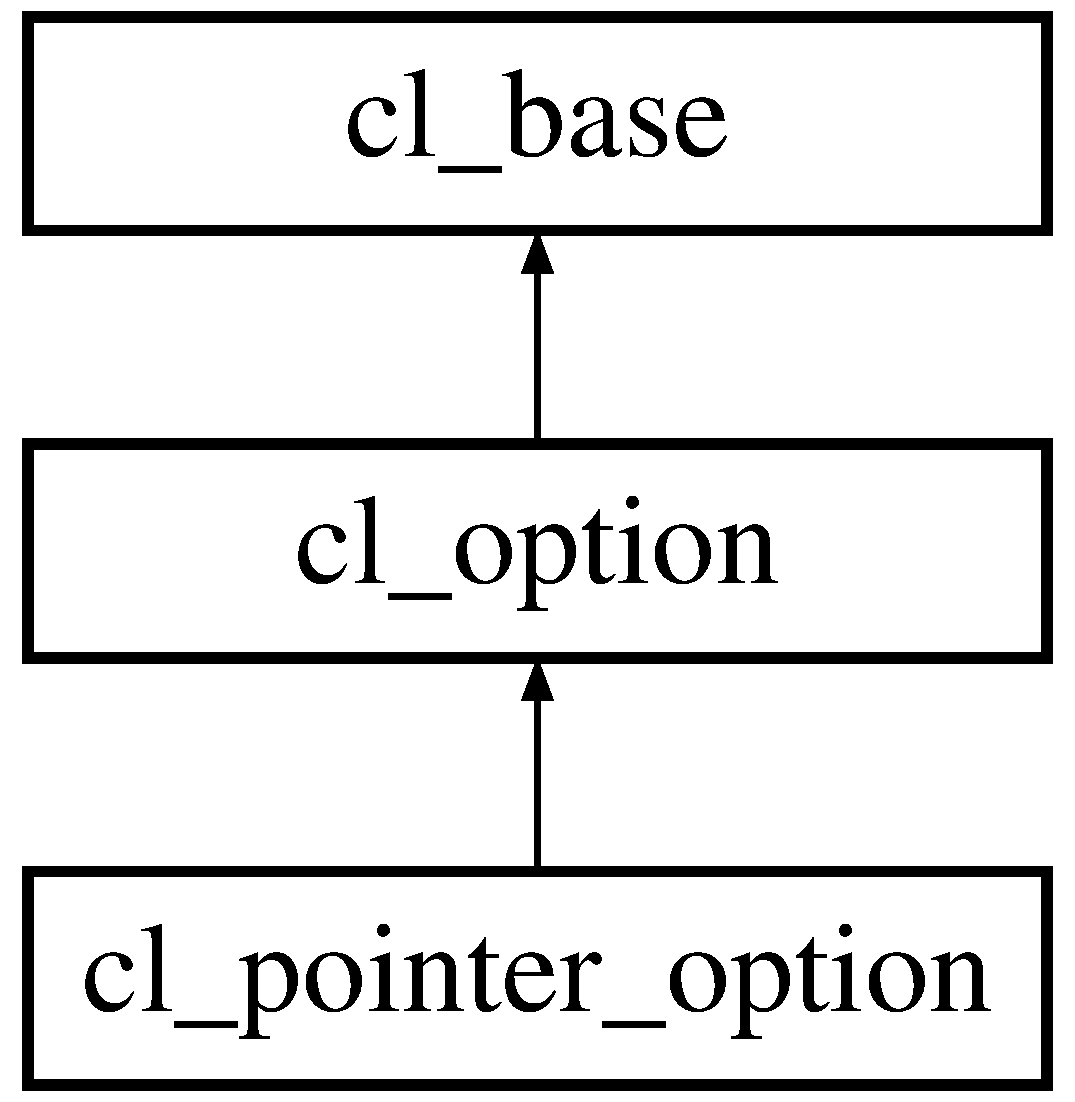
\includegraphics[height=3.000000cm]{classcl__pointer__option}
\end{center}
\end{figure}
\subsection*{Public Member Functions}
\begin{DoxyCompactItemize}
\item 
\hypertarget{classcl__pointer__option_af10fddcb604f7fadde941d2f490c6a0b}{
{\bfseries cl\_\-pointer\_\-option} (class \hyperlink{classcl__base}{cl\_\-base} $\ast$the\_\-creator, char $\ast$aname, char $\ast$Ihelp)}
\label{classcl__pointer__option_af10fddcb604f7fadde941d2f490c6a0b}

\item 
\hypertarget{classcl__pointer__option_a8e5dab7a00f6172e11b8ba49ddb44beb}{
virtual class \hyperlink{classcl__option}{cl\_\-option} \& {\bfseries operator=} (class \hyperlink{classcl__option}{cl\_\-option} \&o)}
\label{classcl__pointer__option_a8e5dab7a00f6172e11b8ba49ddb44beb}

\item 
\hypertarget{classcl__pointer__option_a0dcfc8cbac864eaffd94395b529bfdeb}{
virtual void {\bfseries print} (class cl\_\-console $\ast$con)}
\label{classcl__pointer__option_a0dcfc8cbac864eaffd94395b529bfdeb}

\item 
\hypertarget{classcl__pointer__option_a1fe03453858ddee4ff5b77c6adc2f293}{
virtual char $\ast$ {\bfseries get\_\-type\_\-name} (void)}
\label{classcl__pointer__option_a1fe03453858ddee4ff5b77c6adc2f293}

\end{DoxyCompactItemize}


The documentation for this class was generated from the following files:\begin{DoxyCompactItemize}
\item 
optioncl.h\item 
option.cc\end{DoxyCompactItemize}

\hypertarget{classcl__sorted__list}{
\section{cl\_\-sorted\_\-list Class Reference}
\label{classcl__sorted__list}\index{cl\_\-sorted\_\-list@{cl\_\-sorted\_\-list}}
}
Inheritance diagram for cl\_\-sorted\_\-list:\begin{figure}[H]
\begin{center}
\leavevmode
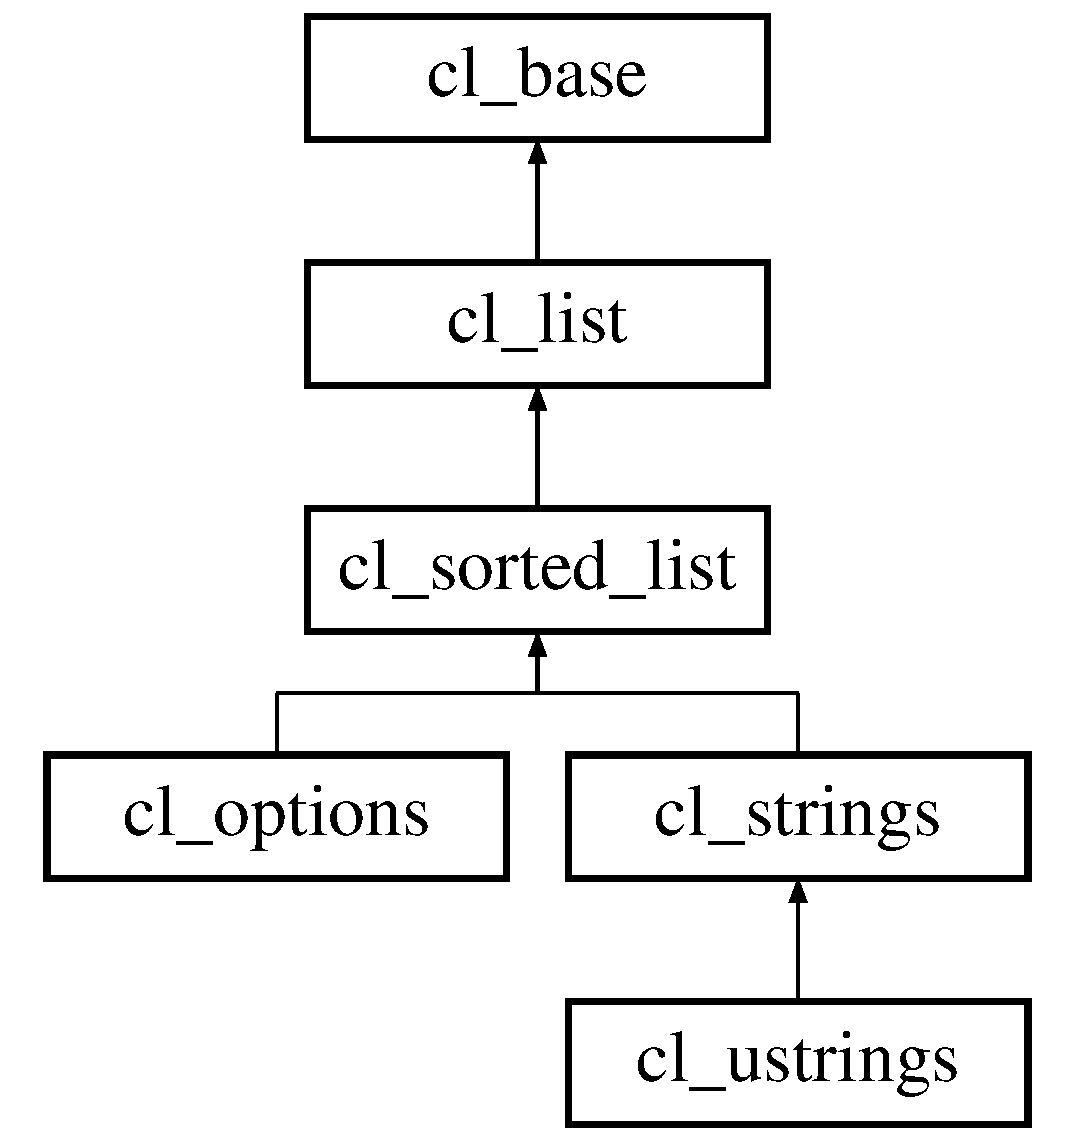
\includegraphics[height=5.000000cm]{classcl__sorted__list}
\end{center}
\end{figure}
\subsection*{Public Member Functions}
\begin{DoxyCompactItemize}
\item 
\hypertarget{classcl__sorted__list_aeb2749fd5bc66a8ea16036e232a531c6}{
{\bfseries cl\_\-sorted\_\-list} (t\_\-index alimit, t\_\-index adelta, char $\ast$aname)}
\label{classcl__sorted__list_aeb2749fd5bc66a8ea16036e232a531c6}

\item 
\hypertarget{classcl__sorted__list_a2a9833376b478fe35673920f53fe890a}{
virtual bool {\bfseries search} (void $\ast$key, t\_\-index \&index)}
\label{classcl__sorted__list_a2a9833376b478fe35673920f53fe890a}

\item 
\hypertarget{classcl__sorted__list_a568582e61a301cdb7692924dbee0b81c}{
virtual t\_\-index {\bfseries index\_\-of} (void $\ast$item)}
\label{classcl__sorted__list_a568582e61a301cdb7692924dbee0b81c}

\item 
\hypertarget{classcl__sorted__list_ac9fbd7c30b40311a02e6a8cfe712e1ad}{
virtual t\_\-index {\bfseries add} (void $\ast$item)}
\label{classcl__sorted__list_ac9fbd7c30b40311a02e6a8cfe712e1ad}

\item 
\hypertarget{classcl__sorted__list_a9b831b68854f23c2f38c05b660f9a3a3}{
virtual void $\ast$ {\bfseries key\_\-of} (void $\ast$item)}
\label{classcl__sorted__list_a9b831b68854f23c2f38c05b660f9a3a3}

\end{DoxyCompactItemize}
\subsection*{Public Attributes}
\begin{DoxyCompactItemize}
\item 
\hypertarget{classcl__sorted__list_a36a95023a06dd3ce8d0977daac39d175}{
bool {\bfseries Duplicates}}
\label{classcl__sorted__list_a36a95023a06dd3ce8d0977daac39d175}

\end{DoxyCompactItemize}


The documentation for this class was generated from the following files:\begin{DoxyCompactItemize}
\item 
pobjcl.h\item 
pobj.cc\end{DoxyCompactItemize}

\hypertarget{classcl__string__option}{
\section{cl\_\-string\_\-option Class Reference}
\label{classcl__string__option}\index{cl\_\-string\_\-option@{cl\_\-string\_\-option}}
}
Inheritance diagram for cl\_\-string\_\-option:\begin{figure}[H]
\begin{center}
\leavevmode
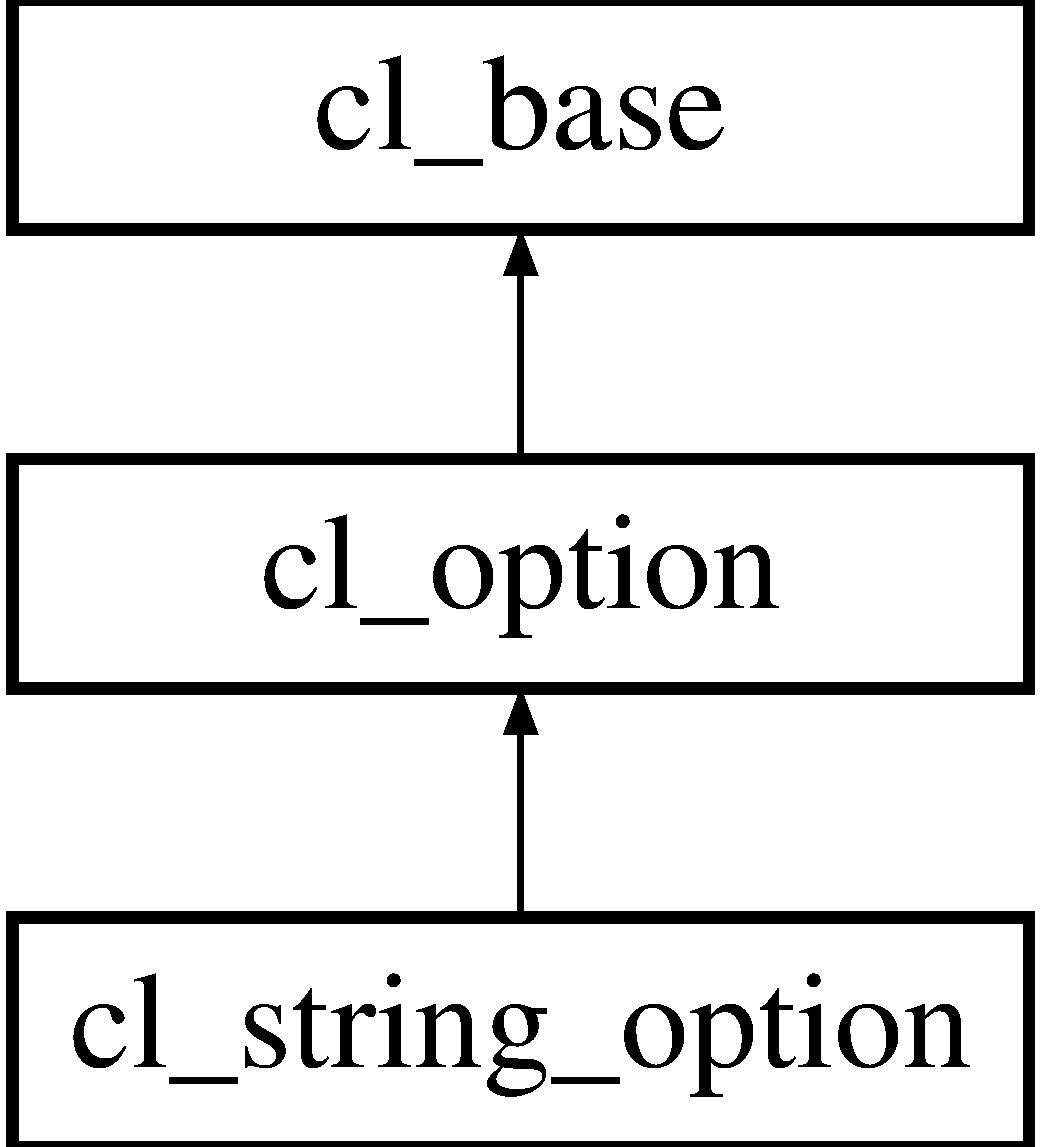
\includegraphics[height=3.000000cm]{classcl__string__option}
\end{center}
\end{figure}
\subsection*{Public Member Functions}
\begin{DoxyCompactItemize}
\item 
\hypertarget{classcl__string__option_ac53f7804fcf03d5dde133c98f656d11c}{
{\bfseries cl\_\-string\_\-option} (class \hyperlink{classcl__base}{cl\_\-base} $\ast$the\_\-creator, char $\ast$aname, char $\ast$Ihelp)}
\label{classcl__string__option_ac53f7804fcf03d5dde133c98f656d11c}

\item 
\hypertarget{classcl__string__option_a95be9951ea38ddb294c0130d4f49c5f5}{
virtual class \hyperlink{classcl__option}{cl\_\-option} \& {\bfseries operator=} (class \hyperlink{classcl__option}{cl\_\-option} \&o)}
\label{classcl__string__option_a95be9951ea38ddb294c0130d4f49c5f5}

\item 
virtual void \hyperlink{classcl__string__option_a4248fdd667d4d76597e69748bab52819}{print} (class cl\_\-console $\ast$con)
\item 
\hypertarget{classcl__string__option_ab0667f92081b84257e5c649a1ac91645}{
virtual char $\ast$ {\bfseries get\_\-type\_\-name} (void)}
\label{classcl__string__option_ab0667f92081b84257e5c649a1ac91645}

\end{DoxyCompactItemize}


\subsection{Member Function Documentation}
\hypertarget{classcl__string__option_a4248fdd667d4d76597e69748bab52819}{
\index{cl\_\-string\_\-option@{cl\_\-string\_\-option}!print@{print}}
\index{print@{print}!cl_string_option@{cl\_\-string\_\-option}}
\subsubsection[{print}]{\setlength{\rightskip}{0pt plus 5cm}void cl\_\-string\_\-option::print (
\begin{DoxyParamCaption}
\item[{class cl\_\-console $\ast$}]{con}
\end{DoxyParamCaption}
)\hspace{0.3cm}{\ttfamily  \mbox{[}virtual\mbox{]}}}}
\label{classcl__string__option_a4248fdd667d4d76597e69748bab52819}


(bool $\ast$)option 



Reimplemented from \hyperlink{classcl__option}{cl\_\-option}.



The documentation for this class was generated from the following files:\begin{DoxyCompactItemize}
\item 
optioncl.h\item 
option.cc\end{DoxyCompactItemize}

\hypertarget{classcl__strings}{
\section{cl\_\-strings Class Reference}
\label{classcl__strings}\index{cl\_\-strings@{cl\_\-strings}}
}
Inheritance diagram for cl\_\-strings:\begin{figure}[H]
\begin{center}
\leavevmode
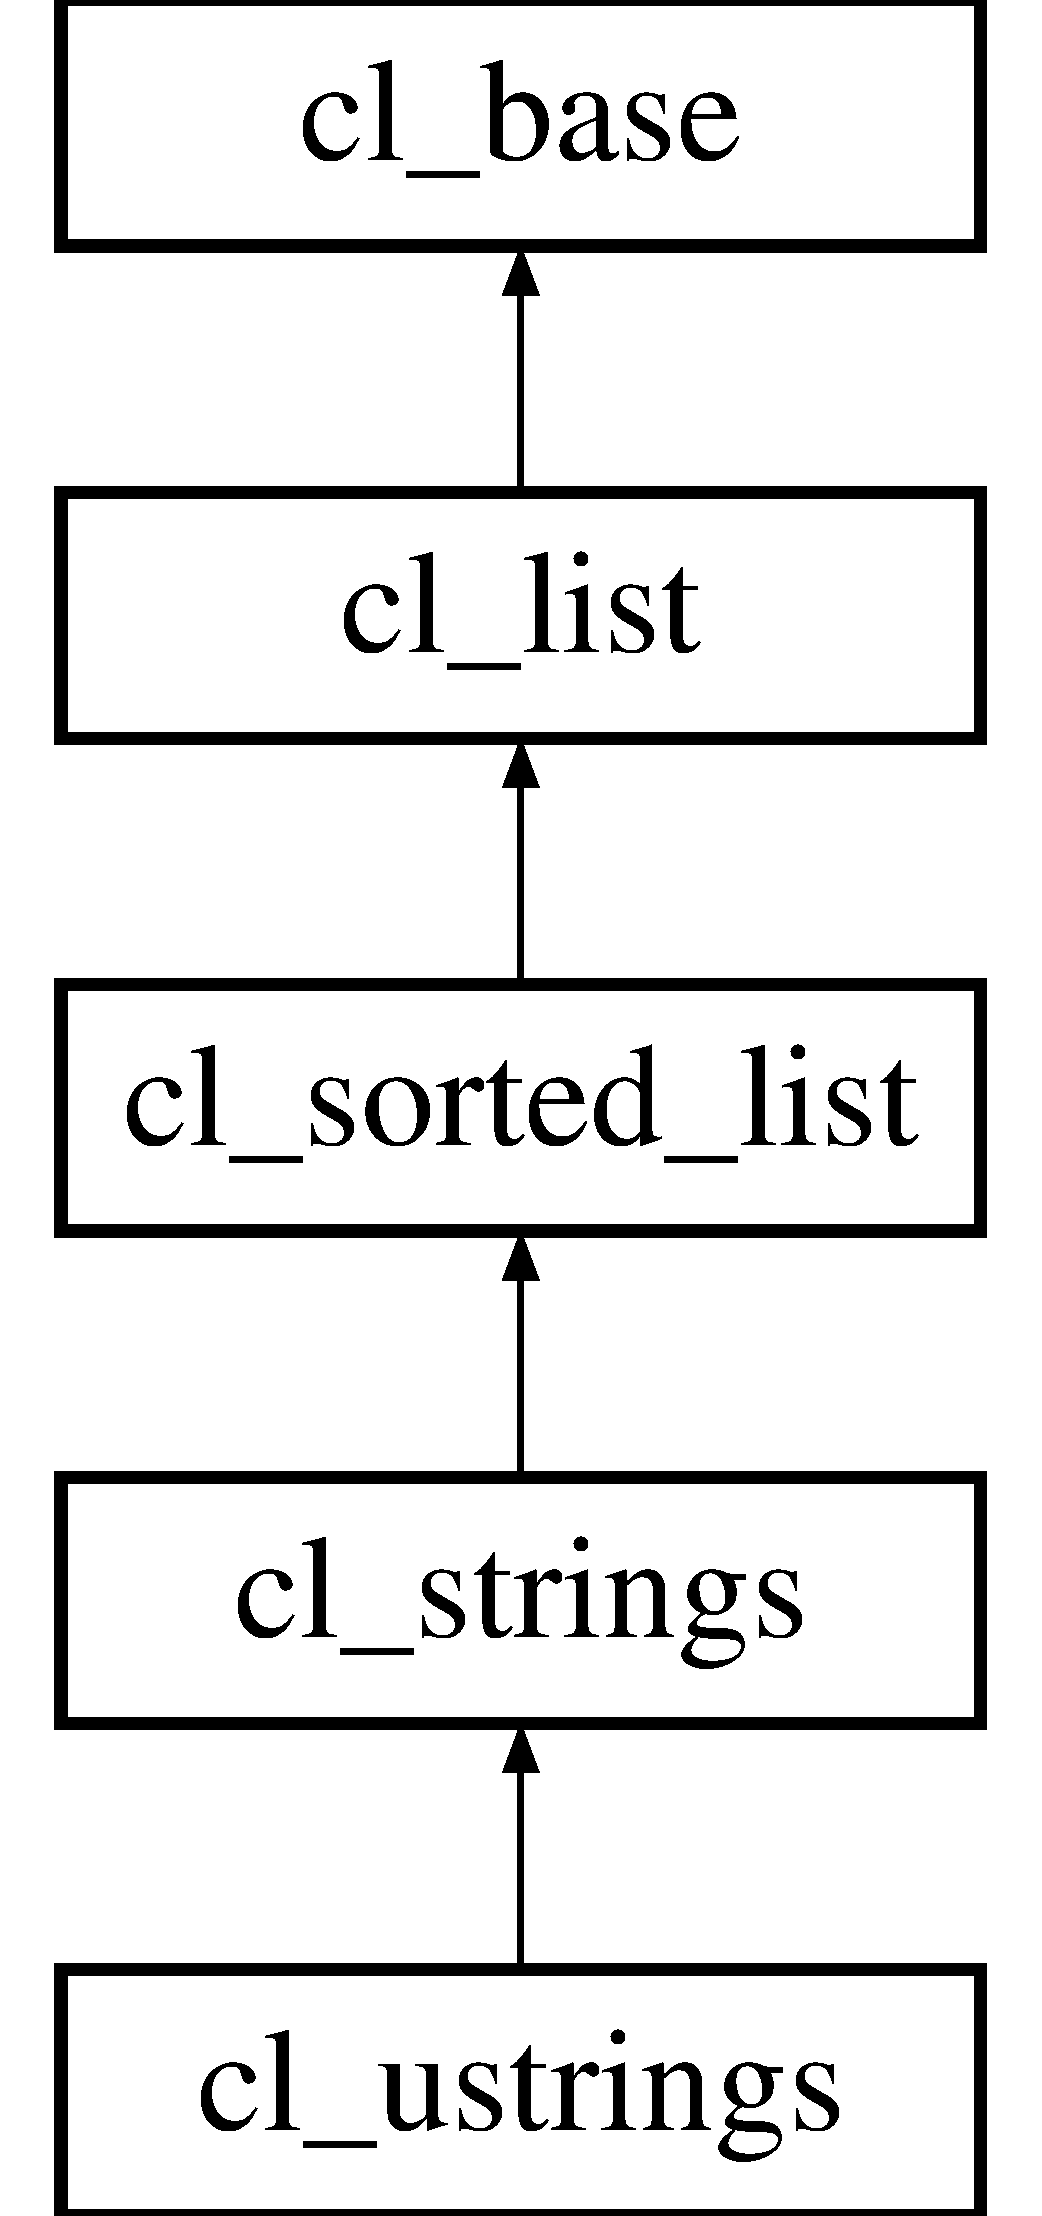
\includegraphics[height=5.000000cm]{classcl__strings}
\end{center}
\end{figure}
\subsection*{Public Member Functions}
\begin{DoxyCompactItemize}
\item 
\hypertarget{classcl__strings_ab64f40558c0308ee24800c1b0a7f7a13}{
{\bfseries cl\_\-strings} (t\_\-index alimit, t\_\-index adelta, char $\ast$aname)}
\label{classcl__strings_ab64f40558c0308ee24800c1b0a7f7a13}

\end{DoxyCompactItemize}


The documentation for this class was generated from the following files:\begin{DoxyCompactItemize}
\item 
pobjcl.h\item 
pobj.cc\end{DoxyCompactItemize}

\hypertarget{classcl__ustrings}{
\section{cl\_\-ustrings Class Reference}
\label{classcl__ustrings}\index{cl\_\-ustrings@{cl\_\-ustrings}}
}
Inheritance diagram for cl\_\-ustrings:\begin{figure}[H]
\begin{center}
\leavevmode
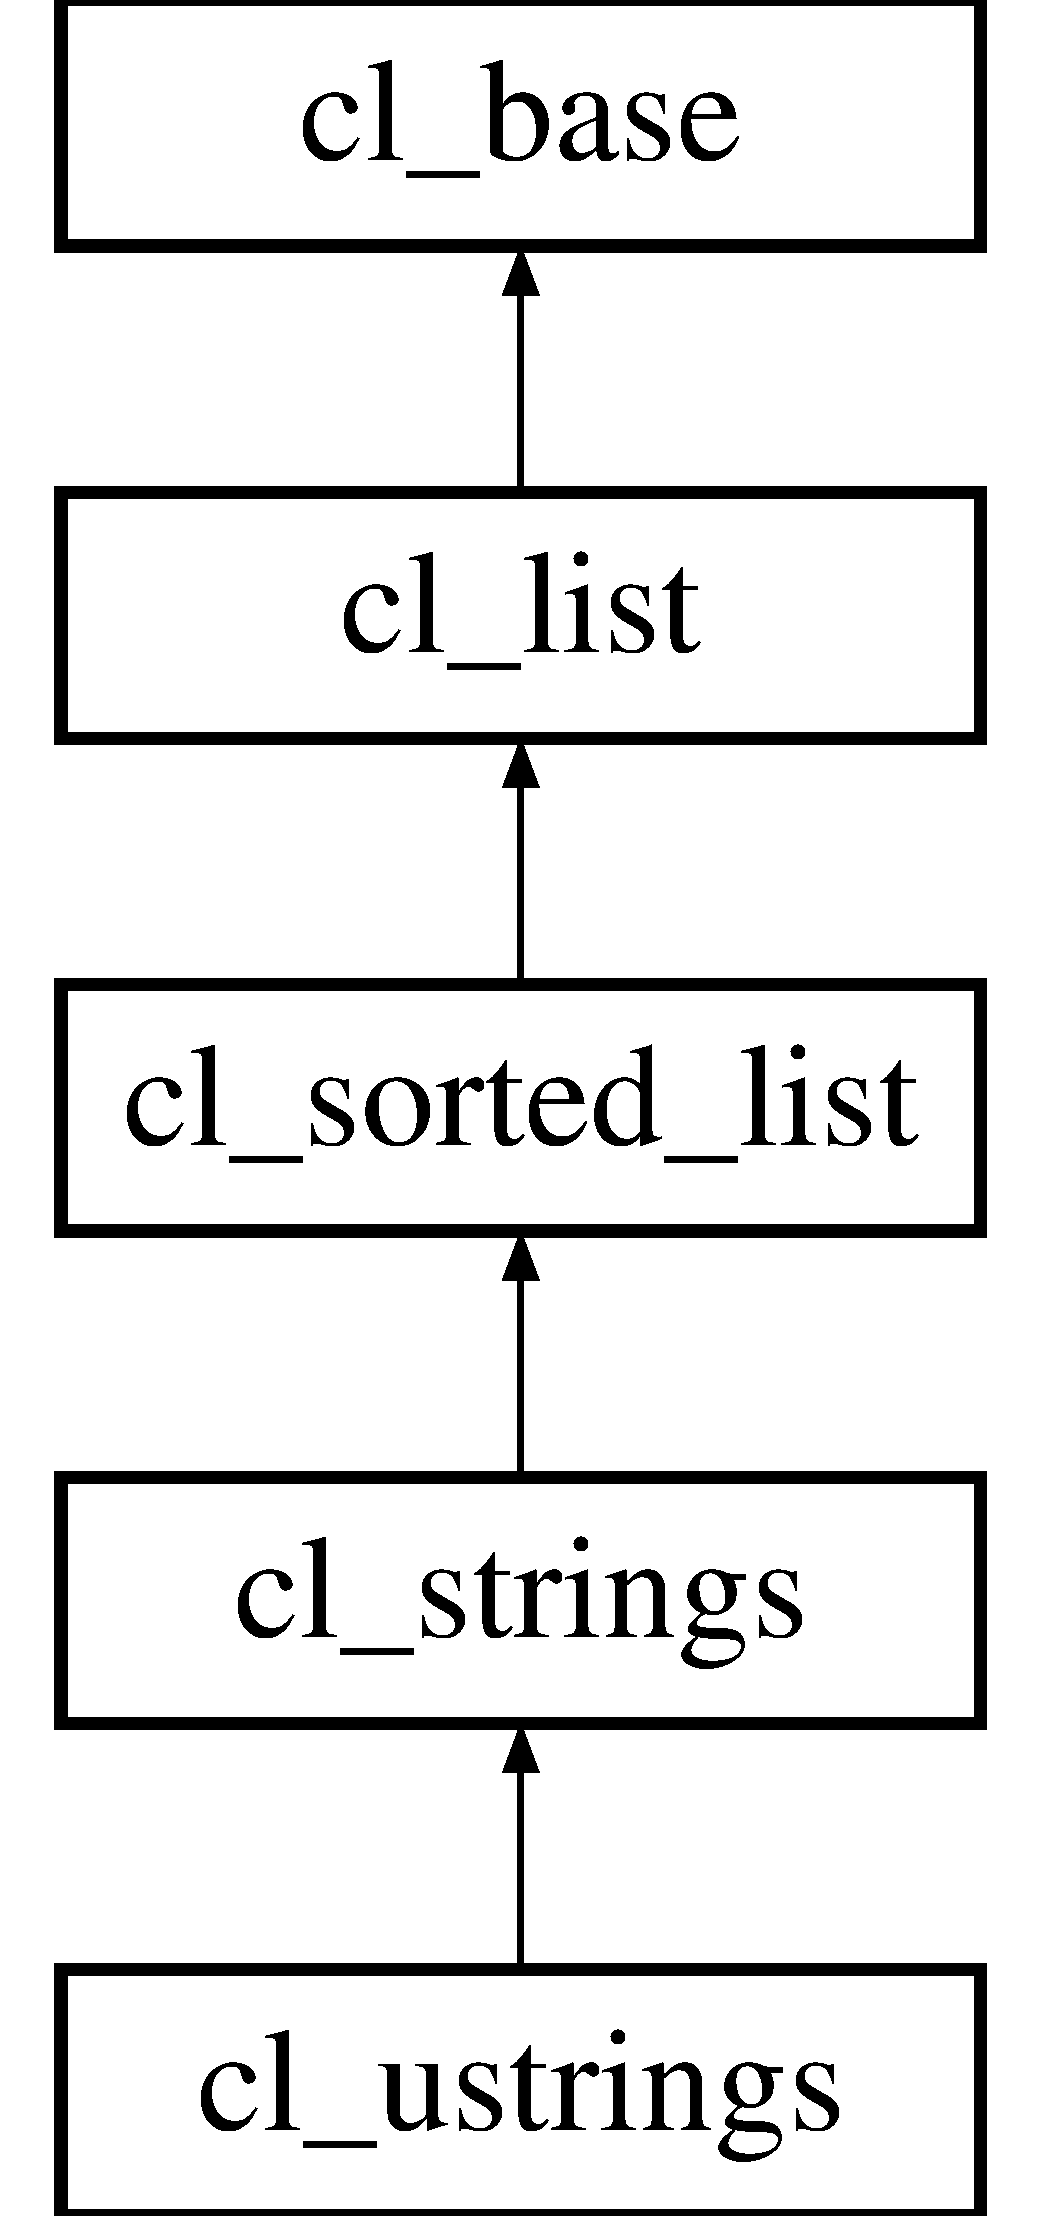
\includegraphics[height=5.000000cm]{classcl__ustrings}
\end{center}
\end{figure}
\subsection*{Public Member Functions}
\begin{DoxyCompactItemize}
\item 
\hypertarget{classcl__ustrings_af2bd507c937c5c80a8571115519f93a1}{
{\bfseries cl\_\-ustrings} (t\_\-index alimit, t\_\-index adelta, char $\ast$aname)}
\label{classcl__ustrings_af2bd507c937c5c80a8571115519f93a1}

\end{DoxyCompactItemize}


The documentation for this class was generated from the following files:\begin{DoxyCompactItemize}
\item 
pobjcl.h\item 
pobj.cc\end{DoxyCompactItemize}

\hypertarget{structcpu__entry}{
\section{cpu\_\-entry Struct Reference}
\label{structcpu__entry}\index{cpu\_\-entry@{cpu\_\-entry}}
}
\subsection*{Public Attributes}
\begin{DoxyCompactItemize}
\item 
\hypertarget{structcpu__entry_abd35b264b163d64830ef9f5daae102a8}{
char $\ast$ {\bfseries type\_\-str}}
\label{structcpu__entry_abd35b264b163d64830ef9f5daae102a8}

\item 
\hypertarget{structcpu__entry_a0dee5cc2b42478b805b7fa17ce14b010}{
int {\bfseries type}}
\label{structcpu__entry_a0dee5cc2b42478b805b7fa17ce14b010}

\item 
\hypertarget{structcpu__entry_a3d3710e3547ce9b64d919bda6feb0a57}{
int {\bfseries technology}}
\label{structcpu__entry_a3d3710e3547ce9b64d919bda6feb0a57}

\end{DoxyCompactItemize}


The documentation for this struct was generated from the following file:\begin{DoxyCompactItemize}
\item 
stypes.h\end{DoxyCompactItemize}

\hypertarget{structdis__entry}{
\section{dis\_\-entry Struct Reference}
\label{structdis__entry}\index{dis\_\-entry@{dis\_\-entry}}
}
\subsection*{Public Attributes}
\begin{DoxyCompactItemize}
\item 
\hypertarget{structdis__entry_a0eefc2c174f1c38d4119a371431440bf}{
uint {\bfseries code}}
\label{structdis__entry_a0eefc2c174f1c38d4119a371431440bf}

\item 
\hypertarget{structdis__entry_ac0dde18f7f844e57386791b1324ebdca}{
uint {\bfseries mask}}
\label{structdis__entry_ac0dde18f7f844e57386791b1324ebdca}

\item 
\hypertarget{structdis__entry_a27b5ed80ac1be7cee1d44a61501b5082}{
char {\bfseries branch}}
\label{structdis__entry_a27b5ed80ac1be7cee1d44a61501b5082}

\item 
\hypertarget{structdis__entry_a6e9084d688366103cfdd5cedb061df9c}{
uchar {\bfseries length}}
\label{structdis__entry_a6e9084d688366103cfdd5cedb061df9c}

\item 
\hypertarget{structdis__entry_a1294a8cfe957e332f4f267c960ea6e73}{
char $\ast$ {\bfseries mnemonic}}
\label{structdis__entry_a1294a8cfe957e332f4f267c960ea6e73}

\end{DoxyCompactItemize}


The documentation for this struct was generated from the following file:\begin{DoxyCompactItemize}
\item 
stypes.h\end{DoxyCompactItemize}

\hypertarget{structid__element}{
\section{id\_\-element Struct Reference}
\label{structid__element}\index{id\_\-element@{id\_\-element}}
}
\subsection*{Public Attributes}
\begin{DoxyCompactItemize}
\item 
\hypertarget{structid__element_a05f6fa143d9737875b46857e20fad99c}{
int {\bfseries id}}
\label{structid__element_a05f6fa143d9737875b46857e20fad99c}

\item 
\hypertarget{structid__element_a7bc9456f4d0a0ad95d6c63f12f97dda0}{
char $\ast$ {\bfseries id\_\-string}}
\label{structid__element_a7bc9456f4d0a0ad95d6c63f12f97dda0}

\end{DoxyCompactItemize}


The documentation for this struct was generated from the following file:\begin{DoxyCompactItemize}
\item 
stypes.h\end{DoxyCompactItemize}

\hypertarget{structinput__args}{
\section{input\_\-args Struct Reference}
\label{structinput__args}\index{input\_\-args@{input\_\-args}}
}
\subsection*{Public Attributes}
\begin{DoxyCompactItemize}
\item 
\hypertarget{structinput__args_acce29ac1b53176d1378cd032cd91a81e}{
int {\bfseries nr}}
\label{structinput__args_acce29ac1b53176d1378cd032cd91a81e}

\item 
\hypertarget{structinput__args_a7008972ceaca6361b86786d904af32d8}{
char $\ast$ {\bfseries fin\_\-name}}
\label{structinput__args_a7008972ceaca6361b86786d904af32d8}

\item 
\hypertarget{structinput__args_a7db8d3978c4f03d0790ff252e59daffe}{
char $\ast$ {\bfseries fout\_\-name}}
\label{structinput__args_a7db8d3978c4f03d0790ff252e59daffe}

\end{DoxyCompactItemize}


The documentation for this struct was generated from the following file:\begin{DoxyCompactItemize}
\item 
ptt.cc\end{DoxyCompactItemize}

\hypertarget{structname__entry}{
\section{name\_\-entry Struct Reference}
\label{structname__entry}\index{name\_\-entry@{name\_\-entry}}
}
\subsection*{Public Attributes}
\begin{DoxyCompactItemize}
\item 
\hypertarget{structname__entry_abead9150b877dbc54ebab7fa819042b1}{
int {\bfseries cpu\_\-type}}
\label{structname__entry_abead9150b877dbc54ebab7fa819042b1}

\item 
\hypertarget{structname__entry_a715ec77ecc2ba2e10811681c269a2437}{
t\_\-addr {\bfseries addr}}
\label{structname__entry_a715ec77ecc2ba2e10811681c269a2437}

\item 
\hypertarget{structname__entry_a4a70896a15e2b5f16e685903d25c247b}{
char $\ast$ {\bfseries name}}
\label{structname__entry_a4a70896a15e2b5f16e685903d25c247b}

\end{DoxyCompactItemize}


The documentation for this struct was generated from the following file:\begin{DoxyCompactItemize}
\item 
stypes.h\end{DoxyCompactItemize}

\hypertarget{unionoption__value}{
\section{option\_\-value Union Reference}
\label{unionoption__value}\index{option\_\-value@{option\_\-value}}
}
\subsection*{Public Attributes}
\begin{DoxyCompactItemize}
\item 
\hypertarget{unionoption__value_a9aac131c9b94b22baa25ca7bd577aa79}{
long {\bfseries ival}}
\label{unionoption__value_a9aac131c9b94b22baa25ca7bd577aa79}

\item 
\hypertarget{unionoption__value_a04b0aca89c7a7d36a3614d77e764538b}{
double {\bfseries fval}}
\label{unionoption__value_a04b0aca89c7a7d36a3614d77e764538b}

\item 
\hypertarget{unionoption__value_ae2f3b780312ac1c942829543cc939a73}{
bool {\bfseries bval}}
\label{unionoption__value_ae2f3b780312ac1c942829543cc939a73}

\item 
\hypertarget{unionoption__value_abf07543ff683523252d1109afa373348}{
char $\ast$ {\bfseries sval}}
\label{unionoption__value_abf07543ff683523252d1109afa373348}

\item 
\hypertarget{unionoption__value_ace848858c052f23be603a63780ebbbae}{
void $\ast$ {\bfseries pval}}
\label{unionoption__value_ace848858c052f23be603a63780ebbbae}

\end{DoxyCompactItemize}


The documentation for this union was generated from the following file:\begin{DoxyCompactItemize}
\item 
optioncl.h\end{DoxyCompactItemize}

\hypertarget{structsim__args}{
\section{sim\_\-args Struct Reference}
\label{structsim__args}\index{sim\_\-args@{sim\_\-args}}
}
\subsection*{Public Attributes}
\begin{DoxyCompactItemize}
\item 
\hypertarget{structsim__args_afcc2130fe3359fd70c3515b13b79918e}{
long int {\bfseries steps2go}}
\label{structsim__args_afcc2130fe3359fd70c3515b13b79918e}

\end{DoxyCompactItemize}


The documentation for this struct was generated from the following file:\begin{DoxyCompactItemize}
\item 
ptt.cc\end{DoxyCompactItemize}

\printindex
\end{document}
